\documentclass[11pt,a4paper,openany]{ctexrep}
\usepackage[a4paper,margin=23mm,headheight=15pt]{geometry}
\usepackage{amsmath,amssymb,mathtools,bm}
\usepackage{siunitx}
\usepackage{booktabs,tabularx,array,longtable}
\usepackage{enumitem}
\usepackage{graphicx}
\usepackage{xcolor}
\usepackage{tikz}
\usepackage{pgfplots}
\pgfplotsset{compat=1.18}
\usetikzlibrary{arrows.meta,positioning,shapes.geometric,calc,fit,decorations.pathmorphing}
\usepackage[most]{tcolorbox}
\usepackage{hyperref}
\usepackage{fancyhdr}
\usepackage{titlesec}
\usepackage{microtype}
\usepackage{setspace}

\definecolor{KidBlue}{HTML}{22577A}
\definecolor{KidTeal}{HTML}{2A9D8F}
\definecolor{KidGold}{HTML}{E9C46A}
\definecolor{KidRed}{HTML}{C8553D}
\definecolor{KidGray}{HTML}{F3F5F7}
\definecolor{KidDark}{HTML}{263238}

\hypersetup{colorlinks=true,linkcolor=KidBlue,urlcolor=KidBlue,citecolor=KidTeal,pdftitle={KID入门讲义 v0.6},pdfauthor={ChatGPT 辅助整理}}
\setstretch{1.15}
\setlist[itemize]{leftmargin=2em,itemsep=0.25em,topsep=0.4em}
\setlist[enumerate]{leftmargin=2em,itemsep=0.25em,topsep=0.4em}
\setlength{\parindent}{2em}
\setlength{\parskip}{0.25em}

\pagestyle{fancy}
\fancyhf{}
\fancyhead[L]{KID 入门讲义 v0.6}
\fancyhead[R]{\leftmark}
\fancyfoot[C]{\thepage}
\renewcommand{\headrulewidth}{0.4pt}

\titleformat{\chapter}[display]{\bfseries\Huge\color{KidDark}}{\filleft\color{KidBlue}\fontsize{44}{44}\selectfont\thechapter}{1ex}{\titlerule\vspace{1ex}\filright}
\titleformat{\section}{\Large\bfseries\color{KidBlue}}{\thesection}{0.7em}{}
\titleformat{\subsection}{\large\bfseries\color{KidTeal}}{\thesubsection}{0.7em}{}

\newtcolorbox{goalbox}{colback=KidBlue!5,colframe=KidBlue,boxrule=0.8pt,arc=2mm,title=本节目标,fonttitle=\bfseries}
\newtcolorbox{intuitionbox}{colback=KidTeal!6,colframe=KidTeal,boxrule=0.8pt,arc=2mm,title=物理直觉,fonttitle=\bfseries}
\newtcolorbox{projectbox}{colback=KidGold!16,colframe=KidGold!80!black,boxrule=0.8pt,arc=2mm,title=映射到你的 150 GHz LEKID,fonttitle=\bfseries}
\newtcolorbox{mistakebox}{colback=KidRed!5,colframe=KidRed,boxrule=0.8pt,arc=2mm,title=常见误区,fonttitle=\bfseries}
\newtcolorbox{checkpointbox}{colback=KidGray,colframe=KidDark!55,boxrule=0.7pt,arc=2mm,title=理解检查,fonttitle=\bfseries}
\newtcolorbox{formula}[1][]{colback=white,colframe=KidBlue!75,boxrule=0.9pt,arc=1mm,#1}

\newcommand{\qp}{\mathrm{qp}}
\newcommand{\Stwentyone}{S_{21}}
\newcommand{\fzero}{f_0}
\newcommand{\Qi}{Q_i}
\newcommand{\Qc}{Q_c}
\newcommand{\Qr}{Q_r}
\newcommand{\Lk}{L_k}
\newcommand{\Lg}{L_g}


% --- Flow-chart conventions (v0.2) ---
% Solid arrows = causal/signal flow; dashed arrows = parameter influence;
% plain lines = structural/reciprocal coupling. Explicit anchors avoid arrow-box collisions.
\tikzset{
  flowbox/.style={draw=KidDark!70,rounded corners=2mm,align=center,minimum height=10mm,inner sep=4pt,font=\small,fill=white},
  flowarrow/.style={-{Stealth[length=2.3mm,width=1.7mm]},line width=0.85pt,draw=KidBlue,shorten <=1.2pt,shorten >=1.2pt},
  goldarrow/.style={-{Stealth[length=2.3mm,width=1.7mm]},line width=0.85pt,draw=KidGold!75!black,shorten <=1.2pt,shorten >=1.2pt},
  influence/.style={-{Stealth[length=2.0mm,width=1.5mm]},dashed,line width=0.7pt,draw=KidTeal!85!black,shorten <=1.0pt,shorten >=1.0pt},
  structlink/.style={line width=0.8pt,draw=KidBlue!85!black},
  dimline/.style={Stealth-Stealth,thin,draw=KidDark!75}
}

\begin{document}

\begin{titlepage}
\centering
\vspace*{2.2cm}
{\fontsize{30}{38}\selectfont\bfseries\color{KidDark} KID 入门讲义}\par
\vspace{0.5cm}
{\Large\color{KidBlue} 从“一个光子”到可读出的微波信号}\par
\vspace{1.4cm}
{\large Version 0.6 · 2026-09-07}\par
\vfill
\begin{tcolorbox}[width=0.88\textwidth,colback=KidGray,colframe=KidBlue!55,arc=3mm]
\centering
\large
这不是一本“先学完凝聚态物理再碰器件”的教材。\\[0.5em]
它采用器件设计者视角：\\[0.3em]
\textbf{先建立可运行的物理图景，再逐层补上微观理论、公式、仿真与实验。}
\end{tcolorbox}
\vfill
{\large 面向：毫米/亚毫米波 KID / LEKID 初学与器件设计}\par
\end{titlepage}

\tableofcontents
\clearpage

\chapter*{如何使用这份讲义}
\addcontentsline{toc}{chapter}{如何使用这份讲义}
这份讲义按“\textbf{物理因果链}”而不是按学科目录组织。每一章都尽量回答四个问题：
\begin{enumerate}
  \item \textbf{发生了什么？} —— 先建立可视化的物理图景；
  \item \textbf{为什么？} —— 用最少但必要的公式把直觉固定下来；
  \item \textbf{怎么测？} —— 把物理量连接到真实实验中的 $I/Q$、$\Stwentyone$、频移和噪声；
  \item \textbf{与 LEKID 设计有什么关系？} —— 把材料、几何、电磁仿真和读出重新接回同一条链。
\end{enumerate}

当前版本 v0.6 在 v0.5 的基础上继续推进六件事：
\begin{itemize}
  \item 完整保留 v0.1--v0.5 已建立的材料、谐振器与 IQ 读出链条；
  \item 从吸收光功率 $P_{\rm abs}$ 与 pair-breaking efficiency $\eta_{\rm pb}$ 出发，建立 quasiparticle generation 与稳态 $N_{\rm qp}$；
  \item 定义 frequency / dissipation responsivity，并把 $P_{\rm abs}$ 映射到 $\delta f_0$、$\delta Q_i^{-1}$ 与 $\delta S_{21}$；
  \item 引入 quasiparticle lifetime 与 resonator ring-down 两个时间尺度，解释 detector bandwidth；
  \item 建立 PSD / ASD / NEP 的严格单位和 input-referred noise 概念，并给出 photon、GR、TLS、amplifier noise 的工程化比较；
  \item 新增 optical responsivity 与 noise budget 的 Python 示例，为后续真实器件定标做准备。
\end{itemize}
后续版本将进入 LEKID absorber / IDC / polarization / backshort 的电磁设计，再把全部理论映射到当前双偏振 \SI{150}{GHz} 项目。

\chapter{KID 入门的总体路线图}

\section{最终要学会的不是一堆名词，而是一张闭环图}
对于一个真正能够设计、仿真和读出 KID 的研究者，知识最后应当闭合成下面这条链：

\begin{center}
\begin{tikzpicture}[node distance=9mm and 6mm]
\node[flowbox,fill=KidGold!20,minimum width=31mm] (opt) {光场与吸收\\$P_{\rm abs},\nu$};
\node[flowbox,right=of opt,minimum width=36mm] (mat) {超导态与材料响应\\$\Delta,N_{\qp},\sigma_1,\sigma_2,L_k$};
\node[flowbox,right=of mat,minimum width=31mm] (res) {GHz 谐振器\\$f_0,Q_i,Q_c$};
\node[flowbox,right=of res,minimum width=34mm] (read) {读出与灵敏度\\$S_{21},I/Q,$ NEP};
\draw[flowarrow] (opt.east)--(mat.west);
\draw[flowarrow] (mat.east)--(res.west);
\draw[flowarrow] (res.east)--(read.west);

\node[flowbox,below=12mm of opt,fill=KidGray,text width=32mm] (geom) {电磁几何\\meander / backshort\\偏振 / 吸收结构};
\node[flowbox,below=12mm of mat,fill=KidGray,text width=30mm] (proc) {材料与工艺\\$T_c,t,R_\Box$\\薄膜质量};
\node[flowbox,below=12mm of read,fill=KidGray,text width=31mm] (chain) {读出链\\耦合 / 放大\\ADC / DSP};
\draw[influence] (geom.north west) to[bend left=10] node[left,font=\scriptsize]{决定吸收} (opt.south west);
\draw[influence] (geom.north east) to[bend left=15] node[below,font=\scriptsize]{改变 $L_g,C$} (res.south west);
\draw[influence] (proc.north) -- (mat.south);
\draw[influence] (chain.north) -- (read.south);
\end{tikzpicture}
\end{center}

你最终要能够在这张图中从任意一格走到任意一格。例如：
\begin{itemize}
  \item 改变膜厚，为什么会影响吸收、$\Lk$、$Q_i$ 和 responsivity？
  \item 加 backshort，为什么主要先改变毫米波吸收，却最终体现在 GHz 读出端的 $I/Q$ 上？
  \item 为什么同样一个 $\Stwentyone$ notch，可能对应完全不同的光学效率？
\end{itemize}

\section{建议的学习模块}
\renewcommand{\arraystretch}{1.25}
\begin{tabularx}{\textwidth}{>{\bfseries}p{1.5cm} p{4.0cm} X p{2.6cm}}
\toprule
模块 & 核心主题 & 学完后应该能回答的问题 & 典型产出 \\
\midrule
M1 & 从光子到 $\Stwentyone$ & KID 到底怎样把光变成可测的 IQ 变化？ & 因果链 + 极简仿真 \\
M2 & 超导基础 & Cooper pair、能隙、准粒子到底是什么？ & BCS 最小知识集 \\
M3 & 动能电感与复电导 & 为什么超导载流子的惯性等效为电感？$\sigma_1,\sigma_2$ 如何进入器件？ & $L_k$ 推导 + MB 框架 \\
M4 & 微波谐振器 & $Q_i,Q_c,Q_r$、耦合和 IQ 圆分别意味着什么？ & resonator fitting \\
M5 & 光学响应 & 光功率如何映射为 $\Delta f_0$、相位和幅度？ & responsivity 模型 \\
M6 & 噪声与 NEP & 什么时候是 photon-noise limited？TLS、GR、放大器噪声如何比较？ & noise budget \\
M7 & LEKID 电磁设计 & meander 为什么既是 absorber 又是 inductor？IDC、偏振、backshort 如何设计？ & 参数化像素模型 \\
M8 & 阵列与读出 & 如何频分复用数百/数千像素？tone spacing、动态范围如何约束设计？ & readout budget \\
M9 & 仿真与实验 & Sonnet/CST/测量数据各自验证哪一层物理？ & 仿真-测量闭环 \\
M10 & 研究课题化 & 如何从“能工作的 KID”走向可发表的问题？ & 论文问题与验证矩阵 \\
\bottomrule
\end{tabularx}

\section{推荐学习顺序}
不建议一上来死磕 Mattis--Bardeen 积分。更高效的顺序是：
\[
\boxed{
\text{可视化因果链}
\rightarrow
\text{等效电路}
\rightarrow
\text{最小超导理论}
\rightarrow
\text{复电导}
\rightarrow
\text{噪声与光学}
\rightarrow
\text{LEKID 工程设计}
}
\]
这使得每一个新公式都有“它为什么值得学”的位置。

\chapter{从一个光子到 $S_{21}$：KID 的第一性物理图景}

\begin{goalbox}
学完本章后，你应该能不看资料独立讲清：
\begin{enumerate}
  \item 为什么毫米波/亚毫米波光子能够改变超导薄膜；
  \item 为什么这种变化会改变 kinetic inductance 和 microwave loss；
  \item 为什么谐振频率与品质因数因此改变；
  \item 为什么实验最终读到的是 $\Stwentyone=I+jQ$；
  \item 一颗 LEKID 为什么可以同时扮演“光学吸收器”和“GHz 微波谐振器”。
\end{enumerate}
\end{goalbox}

\section{先看全局：KID 是一台“两种频率协同工作”的机器}
KID 初学时最容易混淆的一点，是把“被探测的光”和“用于读出的微波”混为一谈。事实上，它们通常相差几十到上百倍频率。

\begin{center}
\begin{tikzpicture}[node distance=8mm and 9mm]
% Optical / physical-state lane
\node[flowbox,fill=KidGold!23,minimum width=29mm] (ph) {信号辐射\\例如 \SI{150}{GHz}};
\node[flowbox,fill=KidGold!13,right=of ph,minimum width=31mm] (abs) {meander 薄膜\\吸收能量};
\node[flowbox,fill=KidTeal!10,right=of abs,minimum width=31mm] (qp) {$N_{\qp}\uparrow$\\超导态改变};
\node[flowbox,fill=KidBlue!8,right=of qp,minimum width=31mm] (state) {$L_k,Q_i,f_0$\\谐振器状态改变};
\draw[goldarrow] (ph.east)--(abs.west);
\draw[goldarrow] (abs.east)--(qp.west);
\draw[flowarrow] (qp.east)--(state.west);

% Microwave readout lane
\node[flowbox,fill=KidGray,below=18mm of ph,minimum width=29mm] (probe) {GHz probe\\tone source};
\node[flowbox,fill=KidBlue!6,right=of probe,minimum width=34mm] (device) {feedline + KID\\测量 $S_{21}$};
\node[flowbox,fill=KidGray,right=of device,minimum width=31mm] (adc) {低噪声放大\\ADC / DDC};
\node[flowbox,fill=KidBlue!8,right=of adc,minimum width=31mm] (iq) {$I(t),Q(t)$\\数字时间序列};
\draw[flowarrow] (probe.east)--(device.west);
\draw[flowarrow] (device.east)--(adc.west);
\draw[flowarrow] (adc.east)--(iq.west);
\draw[influence] (state.south) -- node[right,font=\scriptsize]{决定 $S_{21}(f)$} (device.north);
\end{tikzpicture}
\end{center}

一句话概括：
\begin{formula}
\[
\boxed{
P_{\rm opt}
\rightarrow N_{\qp}
\rightarrow (L_k,Q_i)
\rightarrow (f_0,Q_r)
\rightarrow S_{21}
\rightarrow I,Q
}
\]
\end{formula}

\begin{intuitionbox}
\textbf{信号光子负责“改变器件”，GHz 探针微波负责“询问器件”。}\\
KID 的巧妙之处，不是把毫米波直接送进 GHz ADC，而是让毫米波先改变一个非常灵敏的超导谐振器，再用微波精确测量这个变化。
\end{intuitionbox}

\section{第一站：入射光子必须有足够的能量}

\subsection{光子的能量尺度}
一个频率为 $\nu$ 的光子能量为
\[
E_\gamma=h\nu.
\]
对于 \SI{150}{GHz}：
\[
E_\gamma = h\nu \approx \SI{9.94e-23}{J}\approx \SI{0.620}{meV}.
\]
这个数本身没有意义，直到我们把它与超导体的能隙 $\Delta$ 比较。

\subsection{超导能隙与 pair-breaking threshold}
在弱耦合 BCS 近似下，零温能隙约为
\[
\Delta(0)\approx1.764\,k_B T_c.
\]
破坏一个 Cooper pair 至少需要产生两个准粒子，因此阈值为
\[
\boxed{h\nu\ge 2\Delta.}
\]
对应的 pair-breaking frequency 近似为
\[
\nu_{\rm pb}=\frac{2\Delta}{h}\approx \SI{73.5}{GHz/K}\times T_c.
\]

\begin{projectbox}
若取铝 $T_c\approx\SI{1.2}{K}$，则
\[
\nu_{\rm pb}\approx\SI{88}{GHz}.
\]
你的目标频率约为 \SI{150}{GHz}，明显高于这个阈值。因此从最基本的能量条件看，\SI{150}{GHz} 光子具备直接 pair breaking 的能力。
\end{projectbox}

\begin{mistakebox}
“光子能量大于 $\Delta$ 就能打碎 Cooper pair”是不准确的。一个 pair 被破坏后对应两个准粒子激发，因此最基本阈值是 $2\Delta$，不是 $\Delta$。
\end{mistakebox}

\section{第二站：Cooper pair 被破坏，准粒子数量上升}

\subsection{现在只需要一个最小的超导图景}
本章暂时不从 BCS 波函数开始。只保留三类对象：
\begin{itemize}
  \item \textbf{Cooper-pair condensate}：超导凝聚态，承担无直流电阻的集体输运；
  \item \textbf{energy gap $\Delta$}：从凝聚态激发出准粒子需要跨越的能量尺度；
  \item \textbf{quasiparticle（准粒子）}：超导体系的激发态，可以参与微波耗散并改变复电导。
\end{itemize}

当一个满足 $h\nu>2\Delta$ 的光子被薄膜吸收后，最简图景是
\[
\gamma + \text{Cooper pair}\rightarrow \qp+\qp.
\]
真实过程还包括高能准粒子的弛豫、声子产生以及二次 pair breaking，因此一个高能光子的能量最终可能形成多个低能准粒子。后续章节会用 pair-breaking efficiency $\eta$ 描述这个过程。

\subsection{为什么天文 LEKID 更适合用“光功率”而不是“一颗光子”思考}
对于连续背景与天文辐射，更合适的动力学图像是
\[
\frac{dN_{\qp}}{dt}=G-R,
\]
其中 $G$ 是准粒子生成率，$R$ 是复合率。持续光照增强通常意味着
\[
P_{\rm opt}\uparrow \Rightarrow G\uparrow \Rightarrow N_{\qp}\uparrow.
\]
因此，本讲义后续更常使用
\[
\boxed{P_{\rm opt}\rightarrow N_{\qp}}
\]
而不是把 LEKID 简化成单光子计数器。

\section{第三站：为什么准粒子增加会影响 kinetic inductance？}

\subsection{先把“动能电感”理解成惯性}
电流意味着载流子有定向运动。载流子有质量，因此它们建立和改变速度需要能量。对于交流电流，这部分能量会周期性地存入和释放。

从电路端看，只要一个元件表现出
\[
V\propto\frac{dI}{dt},
\]
它就具有电感型响应。超导载流子由于惯性产生的这种响应，就是 \textbf{kinetic inductance}。

在一个最简惯性模型中，取有效超导载流子密度为 $n_s$，可得到
\[
L_k\propto\frac{1}{n_s}.
\]
详细推导将在后续“动能电感”章节中完成。这里先抓住因果关系：光照破坏部分凝聚态，使有效超流密度下降，于是同样的交流电流需要更强的载流子速度响应，表现为更大的动能储能和更大的 $L_k$。

\begin{formula}
\[
\boxed{
N_{\qp}\uparrow
\quad\Longrightarrow\quad
n_s\downarrow
\quad\Longrightarrow\quad
L_k\uparrow
}
\]
\end{formula}

\subsection{几何电感与动能电感不是一回事}
KID 的总电感可以写成
\[
L=L_g+L_k.
\]
两者从端口看都像电感，但储能位置不同：

\begin{center}
\begin{tabular}{lll}
\toprule
量 & 主要储能位置 & 直觉 \\
\midrule
$C$ & 电场 & 电荷分离 \\
$L_g$ & 导体周围的磁场 & 电流建立磁场 \\
$L_k$ & 超导载流子的集体动能 & 载流子具有惯性 \\
\bottomrule
\end{tabular}
\end{center}

定义 kinetic inductance fraction
\[
\boxed{\alpha\equiv\frac{L_k}{L_g+L_k}.}
\]
它告诉我们总电感中有多大比例来自对超导态敏感的那部分。$\alpha$ 越大，材料状态变化越容易转化为谐振频率变化；但这并不意味着设计时应无限追求更大的 $\alpha$，因为损耗、非线性、$Q_i$ 和噪声会共同约束器件。

\section{第四站：$L_k$ 的变化如何变成谐振频率变化？}
LEKID 是一个 lumped-element resonator。最简模型为
\[
\boxed{f_0=\frac{1}{2\pi\sqrt{LC}}.}
\]
若光照主要改变 $L_k$ 而几何电感和电容在一阶近似下不变，则
\[
\frac{\delta f_0}{f_0}=-\frac{1}{2}\frac{\delta L}{L}.
\]
又因为
\[
\delta L=\delta L_k,
\]
并利用 $\alpha=L_k/L$，得到
\begin{formula}
\[
\boxed{
\frac{\delta f_0}{f_0}
=-\frac{\alpha}{2}\frac{\delta L_k}{L_k}.
}
\]
\end{formula}
因此最常见的方向是
\[
L_k\uparrow \quad\Rightarrow\quad f_0\downarrow.
\]
这就是“光照使 resonance 向低频移动”的最基础来源。

\begin{checkpointbox}
如果 $L_k$ 占总电感的比例只有 $1\%$，即使 $L_k$ 本身变化明显，总 $L$ 的变化也会被 $L_g$ 稀释。这个事实正是 $\alpha$ 在 KID 设计中如此重要的原因。
\end{checkpointbox}

\section{第五站：准粒子不仅改电感，也会增加耗散}
只看 $L_k$ 还不完整。准粒子数量增加通常也会增强 microwave dissipation，使内部品质因数下降：
\[
N_{\qp}\uparrow\Rightarrow \text{loss}\uparrow\Rightarrow Q_i\downarrow.
\]
因此光照通常同时造成：
\[
\boxed{f_0\text{ 改变}\quad +\quad Q_i\text{ 改变}.}
\]

更微观地，超导薄膜在微波频率下用复电导描述：
\[
\boxed{\sigma=\sigma_1-i\sigma_2.}
\]
在常用约定下，可以先把它记成：
\begin{itemize}
  \item $\sigma_1$：与耗散相关；
  \item $\sigma_2$：与感性/超流响应相关。
\end{itemize}
光照引起的 $N_{\qp}$ 变化会同时改变 $\sigma_1$ 和 $\sigma_2$。这就是以后 Mattis--Bardeen 理论要把“频移”和“损耗变化”统一起来的地方。

\section{第六站：实验为什么最终测 $S_{21}$？}

\subsection{把谐振器挂在一条 microwave feedline 上}
KID 通常通过耦合结构连接到微波传输线。读出系统发送一个 GHz 微波信号，并测量传输系数
\[
\boxed{S_{21}(f)=\frac{V_{\rm out}}{V_{\rm in}}.}
\]
对于最简 notch resonator，可写成
\[
S_{21}(f)=1-\frac{Q_r/Q_c}{1+2jQ_r\dfrac{f-f_0}{f_0}},
\]
并有
\[
\boxed{\frac{1}{Q_r}=\frac{1}{Q_i}+\frac{1}{Q_c}.}
\]
这里：
\begin{itemize}
  \item $Q_i$：内部损耗决定的品质因数；
  \item $Q_c$：与 feedline 耦合强弱决定的品质因数；
  \item $Q_r$：实际观测到的 loaded quality factor。
\end{itemize}

\subsection{扫频阶段：先找到谐振器}
扫过谐振频率时，$|S_{21}|$ 出现 notch。光照改变 $f_0$ 和 $Q_i$，所以 notch 会移动并改变形状。

\begin{center}
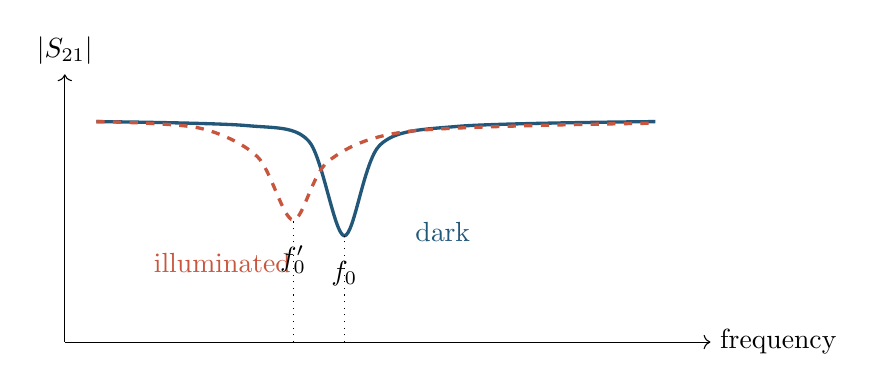
\begin{tikzpicture}[x=1cm,y=1cm]
\draw[->] (0,0)--(8.2,0) node[right]{frequency};
\draw[->] (0,0)--(0,3.4) node[above]{$|S_{21}|$};
\draw[very thick,KidBlue] plot[smooth] coordinates {(0.4,2.8)(2.3,2.75)(3.1,2.55)(3.55,1.35)(4.0,2.5)(5.0,2.74)(7.5,2.8)};
\draw[very thick,KidRed,dashed] plot[smooth] coordinates {(0.4,2.8)(1.7,2.72)(2.45,2.35)(2.9,1.55)(3.35,2.3)(4.4,2.68)(7.5,2.78)};
\node[KidBlue] at (4.8,1.4) {dark};
\node[KidRed] at (2.0,1.0) {illuminated};
\draw[dotted] (3.55,0)--(3.55,1.35) node[below,yshift=-2mm]{$f_0$};
\draw[dotted] (2.9,0)--(2.9,1.55) node[below,yshift=-2mm]{$f_0'$};
\end{tikzpicture}
\end{center}

\subsection{真正观测时：通常固定 probe tone，不需要不停扫频}
实际读出往往选取 $f_{\rm probe}\approx f_0$，持续测量一个复数：
\[
\boxed{S_{21}(t)=I(t)+jQ(t).}
\]
当谐振器因光照发生轻微移动时，固定 probe tone 在 resonance 曲线上的相对位置发生变化，因此 $I$ 和 $Q$ 随时间变化。

\begin{center}
\begin{tikzpicture}[scale=1.05]
\draw[->] (-2.6,0)--(2.8,0) node[right]{$I$};
\draw[->] (0,-2.3)--(0,2.5) node[above]{$Q$};
\draw[very thick,KidBlue] (0.35,0.05) circle (1.55);
\fill[KidBlue] (1.05,1.42) circle (2pt) node[above right]{dark operating point};
\fill[KidRed] (0.72,1.55) circle (2pt) node[above left]{illuminated};
\draw[-{Latex[length=2mm]},very thick,KidRed] (1.05,1.42)--(0.72,1.55);
\node[align=center] at (-1.4,-1.55) {扫频时形成\\近似 IQ 圆};
\end{tikzpicture}
\end{center}

这一步把 KID 与熟悉的数字接收机世界连接起来：最终进入 ADC/DSP 的不是“光子”本身，而是经过谐振器转导后的复基带响应。

\section{为什么读出微波不会自己把 Cooper pair 大量打碎？}
KID 中通常同时存在两种频率尺度：
\begin{align*}
\nu_{\rm signal} &\sim \text{几十到数百 GHz（毫米/亚毫米波）},\\
\nu_{\rm readout} &\sim \text{几百 MHz 到数 GHz（微波）}.
\end{align*}
设计上常希望
\[
h\nu_{\rm readout}<2\Delta,
\]
使单个 readout photon 的能量低于直接 pair-breaking threshold；与此同时
\[
h\nu_{\rm signal}>2\Delta,
\]
使目标光子能够被探测。

\begin{mistakebox}
“读出微波完全不影响超导态”也过于绝对。虽然单个低频 readout photon 通常不能直接 pair break，但过高读出功率仍会引起谐振器非线性、加热、准粒子分布变化等效应。因此实际系统存在最佳 readout power，而不是越大越好。
\end{mistakebox}

\section{LEKID 为什么尤其漂亮：同一块 meander 做两份工作}

\begin{center}
\begin{tikzpicture}[node distance=10mm and 13mm]
\node[flowbox,fill=KidGold!18,minimum width=31mm] (rad) {\SI{150}{GHz}\\入射辐射};
\node[flowbox,fill=KidTeal!10,right=of rad,minimum width=42mm,minimum height=16mm] (mea) {meander inductor\\毫米波 absorber\\GHz kinetic inductor};
\node[flowbox,fill=KidBlue!8,right=18mm of mea,minimum width=31mm,minimum height=16mm] (idc) {IDC\\capacitor};
\draw[goldarrow] (rad.east)--node[above,font=\scriptsize]{光学吸收} (mea.west);
\draw[structlink] (mea.east)--(idc.west);
\node[draw=KidBlue!45,rounded corners=3mm,inner sep=4mm,fit=(mea)(idc),label={[font=\scriptsize,text=KidBlue]above:同一个 GHz LC resonator}] (resgroup) {};

\node[flowbox,fill=KidGray,below=17mm of idc,minimum width=34mm] (cpl) {耦合结构\\$Q_c$};
\node[flowbox,fill=KidGray,left=of cpl,minimum width=42mm] (feed) {feedline\\GHz probe $\rightarrow$ output};
\draw[structlink,dashed] (cpl.north)--node[right,font=\scriptsize]{互易耦合} (resgroup.south east);
\draw[structlink] (feed.east)--(cpl.west);
\end{tikzpicture}
\end{center}

在 LEKID 中，lumped inductor 的 meander 往往同时承担：
\begin{enumerate}
  \item \textbf{毫米波/亚毫米波 absorber}：入射场在图形化薄膜中驱动高频电流并沉积能量；
  \item \textbf{GHz resonator 的电感}：其 $L_g+L_k$ 与 IDC 共同决定微波共振。
\end{enumerate}
因此，毫米波光学设计和 GHz 谐振器设计并不是两个独立问题；它们通过同一块超导薄膜耦合在一起。

\begin{projectbox}
对你的双偏振直接吸收 LEKID，今后每次看一个几何结构都可以问两个问题：\\
\textbf{光学问题：}它如何改变 \SI{150}{GHz} 场、电流分布、吸收和偏振选择性？\\
\textbf{读出问题：}它如何改变 $L_g$、$L_k$、$C$、$f_0$、$Q_i$、$Q_c$ 和可读出性？\\
这两个视角同时成立，才算真正理解 LEKID 几何设计。
\end{projectbox}

\section{把全章压缩成一张“因果链地图”}

\begin{center}
\begin{tikzpicture}[node distance=6mm and 13mm]
\node[flowbox,fill=KidGold!18,minimum width=58mm] (a) {$h\nu>2\Delta$\\信号功率被超导薄膜吸收};
\node[flowbox,below=of a,minimum width=58mm] (b) {Cooper pairs 被激发/破坏\\$N_{\qp}\uparrow$};
\node[flowbox,below=of b,minimum width=58mm] (c) {复电导与表面阻抗改变\\$\sigma_1,\sigma_2$ 改变};
\node[flowbox,fill=KidTeal!8,below left=8mm and 7mm of c,minimum width=45mm] (d1) {感性支路\\$L_k\uparrow$};
\node[flowbox,fill=KidTeal!8,below right=8mm and 7mm of c,minimum width=45mm] (d2) {耗散支路\\loss$\uparrow$, $Q_i\downarrow$};
\node[flowbox,fill=KidBlue!7,below=22mm of c,minimum width=66mm] (e) {谐振器响应改变\\$f_0$ 移动，notch 宽度/深度改变};
\node[flowbox,fill=KidBlue!7,below=of e,minimum width=66mm] (f) {固定 GHz probe tone\\所见 $S_{21}(t)$ 改变};
\node[flowbox,fill=KidGray,below=of f,minimum width=66mm] (g) {$I(t),Q(t)$\\数字后端估计光学信号};
\draw[flowarrow] (a.south)--(b.north);
\draw[flowarrow] (b.south)--(c.north);
\draw[flowarrow] (c.south west) to[out=-90,in=90] (d1.north);
\draw[flowarrow] (c.south east) to[out=-90,in=90] (d2.north);
\draw[flowarrow] (d1.south) to[out=-90,in=155] (e.north west);
\draw[flowarrow] (d2.south) to[out=-90,in=25] (e.north east);
\draw[flowarrow] (e.south)--(f.north);
\draw[flowarrow] (f.south)--(g.north);
\end{tikzpicture}
\end{center}

\section{本章的“公式阶梯”}
第一遍学习只需要按下面顺序记忆，不需要同时掌握所有微观细节。

\begin{enumerate}
  \item 光子能量：
  \[
  E_\gamma=h\nu.
  \]
  \item Pair-breaking threshold：
  \[
  h\nu\ge2\Delta,
  \qquad
  \Delta(0)\approx1.764k_BT_c.
  \]
  \item 动能电感的核心比例关系：
  \[
  L_k\propto\frac1{n_s}.
  \]
  \item LC resonance：
  \[
  f_0=\frac1{2\pi\sqrt{LC}},\qquad L=L_g+L_k.
  \]
  \item 小信号频移：
  \[
  \frac{\delta f_0}{f_0}=-\frac{\alpha}{2}\frac{\delta L_k}{L_k}.
  \]
  \item 品质因数关系：
  \[
  \frac1{Q_r}=\frac1{Q_i}+\frac1{Q_c}.
  \]
  \item 实验读出量：
  \[
  S_{21}=I+jQ.
  \]
\end{enumerate}

\section{六个最容易形成的错误直觉}
\begin{enumerate}
  \item \textbf{“KID 直接测光子的电信号。”}\\
  不对。光先改变超导材料，再改变谐振器，最后才改变微波传输。
  \item \textbf{“只要 $h\nu>\Delta$ 就可以 pair break。”}\\
  基本阈值应是 $2\Delta$。
  \item \textbf{“Kinetic inductance 就是导线弯弯曲曲形成的电感。”}\\
  不对。弯曲几何主要影响 $L_g$；$L_k$ 来自超导载流子的惯性。
  \item \textbf{“光照只是让 resonance 左移。”}\\
  不完整。它通常也改变损耗和 $Q_i$。
  \item \textbf{“KID 工作时必须持续扫频。”}\\
  通常扫频用于定位与标定，真正时间序列读出常使用固定 probe tones。
  \item \textbf{“读出功率越大，SNR 一定越好。”}\\
  不对。过强驱动会进入非线性、加热或改变准粒子状态。
\end{enumerate}

\section{Day 1 的 3--4 小时任务}
如果今天只围绕这一章学习，建议按以下顺序：

\begin{tabularx}{\textwidth}{p{1.8cm} X X}
\toprule
时间 & 任务 & 完成标准 \\
\midrule
35 min & 手画“光子 $\rightarrow$ IQ”因果链，并写出每一箭头为什么成立 & 不看讲义可口述完整链条 \\
45 min & 独立重算 Al 在 $T_c=\SI{1.2}{K}$ 时的 $\Delta$、$2\Delta$ 和 $\nu_{\rm pb}$；再算 \SI{150}{GHz} 光子能量 & 能判断某个频率是否满足 pair-breaking 条件 \\
55 min & 从 $f_0=1/(2\pi\sqrt{LC})$ 推导小信号 $\delta f_0/f_0$，理解 $\alpha$ 的意义 & 推导不用背结果 \\
60 min & Python 画 notch resonator 的 $|S_{21}|$ 与 IQ 圆；令 $f_0$ 左移并比较固定 probe tone 的 $\Delta I,\Delta Q$ & 得到至少 3 张图 \\
30 min & 阅读 Day 2003 的摘要/图 1，并回看本章因果链 & 能指出论文实验的“被测量量”在哪里 \\
20 min & 闭卷回答本章 8 道题 & 至少 6 题能完整解释“为什么” \\
\bottomrule
\end{tabularx}

\section{闭卷理解检查}
\begin{checkpointbox}
不查资料，尝试回答：
\begin{enumerate}
  \item 为什么 pair-breaking threshold 是 $2\Delta$？
  \item 为什么 \SI{150}{GHz} 对 Al 是一个合理的 pair-breaking 频率，而 \SI{5}{GHz} 通常不是？
  \item $N_{\qp}$ 增加后，为什么不能只讨论 $L_k$ 而忽略 $Q_i$？
  \item $L_g$ 与 $L_k$ 的能量分别储存在什么地方？
  \item 为什么 $L_k$ 增加通常导致 $f_0$ 降低？
  \item 什么是 $Q_i,Q_c,Q_r$？
  \item 为什么实际观测可以固定 probe tone，而不必一直扫频？
  \item 用一句完整的话解释：LEKID 的 meander 为什么同时是 absorber 和 resonator inductor？
\end{enumerate}
\end{checkpointbox}

\section{本章结束后你应该拥有的“一个句子”}
如果只能保留一句话，应当是：

\begin{formula}
\centering
\Large
\textbf{KID 用高于能隙阈值的光改变超导薄膜的准粒子与复电导，再用高 $Q$ 微波谐振器把这种微小变化转成可精确测量的 $S_{21}=I+jQ$ 变化。}
\end{formula}


\chapter{动能电感：为什么“载流子的惯性”会变成一个可测的电感？}

\begin{goalbox}
这一章只解决一个核心问题：\textbf{为什么超导载流子的运动惯性可以从器件端口看成一个电感 $L_k$？}
学完后你应能：
\begin{enumerate}
  \item 从 $m\,dv/dt=qE$ 独立推到一段均匀超导条带的 $L_k$；
  \item 用能量法再次得到同一个结果，并解释“电感储能”储在哪里；
  \item 理解 London penetration depth $\lambda_L$ 与 $L_k$ 的关系；
  \item 把三维电感化成薄膜工程中常用的 sheet kinetic inductance $L_{k,\Box}$；
  \item 判断长度、线宽、膜厚、超流密度怎样改变 $L_k$，以及为什么 $\alpha$ 决定频率响应；
  \item 知道电磁仿真中把金属简单设成 PEC 时，哪一部分 KID 物理会被漏掉。
\end{enumerate}
\end{goalbox}

\section{先把“电感”拆成两种储能机制}
对于 LEKID 的一段 meander，总电感可以写成
\[
L=L_g+L_k.
\]
这两个量从端口看都满足“电流变化越快，需要的电压越大”，但物理储能位置不同。

\begin{center}
\begin{tikzpicture}[node distance=10mm and 12mm]
\node[flowbox,fill=KidBlue!6,minimum width=46mm,minimum height=18mm] (c) {$C$：电容\\能量主要储存在电场\\$U_E=\tfrac12CV^2$};
\node[flowbox,fill=KidGold!13,right=of c,minimum width=46mm,minimum height=18mm] (lg) {$L_g$：几何电感\\能量主要储存在磁场\\$U_B=\tfrac12L_gI^2$};
\node[flowbox,fill=KidTeal!10,right=of lg,minimum width=46mm,minimum height=18mm] (lk) {$L_k$：动能电感\\能量储存在载流子动能\\$U_k=\tfrac12L_kI^2$};
\end{tikzpicture}
\end{center}

\begin{intuitionbox}
“meander 弯得很多，所以它有 kinetic inductance”是错误直觉。弯折、回流路径和周围磁场首先影响 $L_g$；$L_k$ 的根源是\textbf{有质量的超导载流子被交流电场加速}。即使一根完全笔直的超导条带，也有 $L_k$。
\end{intuitionbox}

\section{第一条推导：从载流子惯性到 $V=L_k\,dI/dt$}

\subsection{步骤 1：电场使超导载流子加速}
先使用一个故意简化但非常有用的模型。令有效超导载流子的质量、电荷和数密度分别为 $m^*$、$q^*$、$n_s$。忽略散射时，沿导线方向有
\[
m^*\frac{dv}{dt}=q^*E.
\]
电流密度为
\[
J=n_s q^* v.
\]
因此
\[
\frac{dJ}{dt}=n_s q^*\frac{dv}{dt}
=\frac{n_s(q^*)^2}{m^*}E,
\]
从而
\begin{formula}
\[
\boxed{
E=\frac{m^*}{n_s(q^*)^2}\frac{dJ}{dt}
}
\]
\end{formula}

这已经具有“感性”特征：电场不是与 $J$ 本身成正比，而是与 $dJ/dt$ 成正比。

\subsection{步骤 2：从电流密度变成器件端口的电流}
考虑一段长度为 $l$、宽度为 $w$、厚度为 $t$ 的均匀条带，截面积
\[
A=wt.
\]
若电流密度近似均匀，则
\[
J=\frac{I}{A},\qquad V=El.
\]
代入上式：
\[
V=\frac{m^*l}{n_s(q^*)^2A}\frac{dI}{dt}.
\]
与普通电感定义
\[
V=L\frac{dI}{dt}
\]
逐项比较，得到最基础的 kinetic inductance：
\begin{formula}
\[
\boxed{
L_k=\frac{m^*l}{n_s(q^*)^2A}
=\frac{m^*l}{n_s(q^*)^2wt}
}
\]
\end{formula}

\subsection{关于 $2e$、$2m_e$ 与 $n_s$ 的一个重要约定}
有的教材把 $n_s$ 定义为 Cooper-pair density，此时自然使用 $q^*=2e$、$m^*\approx2m_e$；另一些教材把 $n_s$ 写成“参与超流的电子密度”，公式中则使用电子的 $e,m_e$。只要\textbf{密度定义与电荷/质量定义保持一致}，最终物理结果是一致的。初学阶段最危险的是把两套约定混用，从而凭空多出一个 2 或 4 的因子。

\section{第二条推导：用能量法检查结果}
如果前面的代数让你觉得 kinetic inductance 仍然只是“人为定义”，能量法会更直观。

体积 $Al$ 内的超导载流子总动能为
\[
U_k=\frac12(n_sAl)m^*v^2.
\]
又因为
\[
I=J A=n_sq^*vA,
\]
所以
\[
v=\frac{I}{n_sq^*A}.
\]
代回：
\[
U_k
=\frac12\frac{m^*l}{n_s(q^*)^2A}I^2.
\]
而任意等效电感的储能写作
\[
U_L=\frac12LI^2.
\]
因此再次得到
\[
\boxed{L_k=\frac{m^*l}{n_s(q^*)^2A}}.
\]

\begin{checkpointbox}
这两条推导其实在说同一件事：\textbf{建立电流需要让有质量的超导载流子获得速度，因此需要储存动能；而一个端口只要以 $\tfrac12LI^2$ 的形式储能，就会表现为电感。}
\end{checkpointbox}

\section{从公式直接读出四个工程结论}
把
\[
L_k=\frac{m^*l}{n_s(q^*)^2wt}
\]
盯着看，不做任何复杂理论，就已经可以得到：
\begin{enumerate}
  \item \textbf{条带越长，$L_k$ 越大：} $L_k\propto l$；
  \item \textbf{线越窄，$L_k$ 越大：} $L_k\propto1/w$；
  \item \textbf{膜越薄，$L_k$ 越大：} 在均匀电流近似下 $L_k\propto1/t$；
  \item \textbf{超流密度越小，$L_k$ 越大：} $L_k\propto1/n_s$。
\end{enumerate}
最后一条正是 KID 探测原理的核心接口：光照或升温使超导凝聚态被激发，$n_s$ 有效下降，于是 $L_k$ 上升。

\begin{center}
\begin{tikzpicture}[node distance=7mm and 10mm]
\node[flowbox,fill=KidGray,minimum width=32mm] (geom) {几何旋钮\\$l\uparrow,w\downarrow,t\downarrow$};
\node[flowbox,fill=KidGold!13,below=of geom,minimum width=32mm] (state) {材料/状态\\$n_s\downarrow$};
\node[flowbox,fill=KidTeal!10,right=17mm of $(geom)!0.5!(state)$,minimum width=31mm] (lk) {$L_k\uparrow$};
\node[flowbox,fill=KidBlue!7,right=7mm of lk,minimum width=36mm] (alpha) {$\alpha=\dfrac{L_k}{L_g+L_k}$\\通常增大};
\node[flowbox,fill=KidBlue!7,right=7mm of alpha,minimum width=35mm] (resp) {相同材料扰动\\产生更大 $|\delta f_0|$};
\draw[influence] (geom.east) to[bend left=12] (lk.north west);
\draw[influence] (state.east) to[bend right=12] (lk.south west);
\draw[flowarrow] (lk.east)--(alpha.west);
\draw[flowarrow] (alpha.east)--(resp.west);
\end{tikzpicture}
\end{center}

\begin{mistakebox}
“线越窄、膜越薄一定越好”同样不成立。它们虽然能提高 $L_k$ 和潜在 responsivity，却也会改变毫米波表面阻抗匹配、临界电流、非线性、工艺均匀性、损耗和 $Q_i$。KID 设计几乎总是在多目标约束下寻找平衡，而不是最大化单个参数。
\end{mistakebox}

\section{London penetration depth：把 $n_s$ 藏进一个可测的长度尺度}
London 理论把超流密度写进 penetration depth：
\[
\boxed{
\lambda_L^2=\frac{m^*}{\mu_0n_s(q^*)^2}
}
\]
于是前面的均匀电流公式立刻变成
\begin{formula}
\[
\boxed{
L_k=\mu_0\lambda_L^2\frac{l}{A}
=\mu_0\lambda_L^2\frac{l}{wt}
}
\]
\end{formula}
这让一个非常重要的物理事实变得直观：
\[
n_s\downarrow\quad\Longleftrightarrow\quad\lambda_L\uparrow\quad\Longleftrightarrow\quad L_k\uparrow.
\]

\subsection{为什么叫 penetration depth？}
在块体超导体里，微波/磁场并不会像在真空中那样任意深入，而是在表面附近一个特征深度内衰减。$\lambda_L$ 就是描述这种场穿透和超流屏蔽的长度尺度。后续进入复电导与表面阻抗时，我们会看到 $\lambda$、$\sigma_2$ 与 $L_k$ 实际上是同一感性物理的不同语言。

\section{薄膜最实用的语言：每方块动能电感 $L_{k,\Box}$}
对于 KID，我们经常面对几十纳米量级的长而窄薄膜条带。若膜足够薄，使厚度方向电流可以近似均匀，则
\[
L_k=\mu_0\lambda_L^2\frac{l}{wt}
=\left(\mu_0\frac{\lambda_L^2}{t}\right)\frac{l}{w}.
\]
定义
\begin{formula}
\[
\boxed{
L_{k,\Box}\equiv\mu_0\frac{\lambda_L^2}{t}
}
\qquad (t\ll\lambda_L\text{ 的简单 London 极限})
\]
\end{formula}
以及方块数
\[
N_\Box=\frac{l}{w},
\]
就有
\[
\boxed{L_k\approx L_{k,\Box}N_\Box.}
\]

\begin{center}
\begin{tikzpicture}[x=1cm,y=1cm]
\fill[KidTeal!10] (0,0) rectangle (7.2,1.2);
\draw[KidDark!75,line width=0.8pt] (0,0) rectangle (7.2,1.2);
\foreach \x in {1.2,2.4,3.6,4.8,6.0}{\draw[KidDark!35] (\x,0)--(\x,1.2);}
\draw[flowarrow] (-0.8,0.6)--(-0.05,0.6) node[midway,above,font=\scriptsize]{$I$};
\draw[dimline] (0,-0.35)--(7.2,-0.35) node[midway,below,font=\scriptsize]{$l$};
\draw[dimline] (7.55,0)--(7.55,1.2) node[midway,right,font=\scriptsize]{$w$};
\node[font=\small] at (3.6,1.55) {$N_\Box=l/w$：宽度为 $w$ 的“方块”串联};
\end{tikzpicture}
\end{center}

“per square” 很适合平面器件：只要保持材料、膜厚和线宽定义一致，一个长条的总动能电感主要由方块数决定。对于真实 meander，弯角处的 current crowding、邻近导线磁耦合和非均匀电流会让简单 $N_\Box$ 估算产生偏差，因此它是\textbf{手算和设计直觉工具}，不是全波仿真的替代品。

\subsection{膜不再“很薄”时怎么办？}
局域 London 模型下，更一般的表面感性可写成
\[
L_{s}\approx\mu_0\lambda\,\coth\!\left(\frac{t}{\lambda}\right).
\]
当 $t\ll\lambda$ 时，$\coth(t/\lambda)\approx\lambda/t$，便退化到
\[
L_s\approx\mu_0\frac{\lambda^2}{t}.
\]
这里先把它作为“薄膜公式有适用范围”的提醒。真实 KID 薄膜还会受 dirty limit、温度和频率影响；这些会在 Mattis--Bardeen 章节统一处理。

\section{一个数值例子：为什么“每方块几 pH”最后也能变得重要？}
这里故意选一组\textbf{示意参数}，不是在宣称某种特定 Al 薄膜的真实材料常数：
\[
\lambda_{\rm eff}=\SI{200}{nm},\qquad t=\SI{20}{nm}.
\]
则薄膜近似给出
\[
L_{k,\Box}
=\mu_0\frac{\lambda_{\rm eff}^2}{t}
\approx \SI{2.5}{pH}\,/\Box.
\]
如果一段 meander 有约 $1000$ squares，那么仅动能电感就达到
\[
L_k\sim\SI{2.5}{nH}.
\]
这个量级已经足以显著参与 GHz 谐振器总电感。真正器件中必须使用实际薄膜测得或拟合的材料参数（如 $T_c$、$R_\Box$、$\Delta$、$\lambda$）或表面阻抗；不能把这个示意数值直接代入设计。

\section{从 $L_k$ 到 $\alpha$：为什么 KID 要关心“电感里有多少是动能的”}
重新定义
\[
\boxed{
\alpha=\frac{L_k}{L_g+L_k}.
}
\]
若光学扰动主要让 $L_k$ 发生微小变化，而 $L_g$ 和 $C$ 在一阶近似下不变，则
\[
\frac{\delta f_0}{f_0}
=-\frac12\frac{\delta L}{L}
=-\frac12\frac{\delta L_k}{L_g+L_k}.
\]
乘除一个 $L_k$：
\begin{formula}
\[
\boxed{
\frac{\delta f_0}{f_0}
=-\frac{\alpha}{2}\frac{\delta L_k}{L_k}.
}
\]
\end{formula}
所以 $\alpha$ 可以理解为“材料状态变化能够进入总谐振器电感的权重”。如果 $L_g\gg L_k$，材料发生同样的相对变化，却会被大量不敏感的几何电感稀释。

\begin{checkpointbox}
设两颗谐振器的 $\delta L_k/L_k$ 完全相同：A 的 $\alpha=0.05$，B 的 $\alpha=0.5$。在忽略其他差异时，B 的相对频移约为 A 的 10 倍。这并不证明 B 的总 NEP 一定更好，但说明它的\textbf{频率转导增益}更强。
\end{checkpointbox}

\section{对你的 LEKID 几何意味着什么？}
\begin{projectbox}
对你当前的 \SI{150}{GHz} 双偏振直接吸收 LEKID，meander 的线宽、总路径长度和膜厚至少同时参与四件事：
\begin{enumerate}
  \item 决定毫米波表面电流分布和吸收匹配；
  \item 改变几何电感 $L_g$；
  \item 通过 $N_\Box$ 与薄膜参数改变 kinetic inductance $L_k$；
  \item 改变 $\alpha$，进而改变相同超导态扰动造成的 $\delta f_0/f_0$。
\end{enumerate}
所以“把 meander 线做细一点”不是单纯的 GHz 谐振频率调参，也不是单纯的毫米波吸收调参，而是在同时改动两个频率域。
\end{projectbox}

\section{一个与 Sonnet/CST 直接相关的提醒：PEC 会漏掉什么？}
如果在电磁仿真里把超导薄膜完全当作 perfect electric conductor（PEC），求解器仍然可以计算：
\begin{itemize}
  \item 几何电容和大部分 $L_g$；
  \item 电流路径、耦合、辐射和很多几何效应；
  \item 在相应模型下的毫米波场分布。
\end{itemize}
但一个理想 PEC 本身没有“载流子惯性对应的表面感抗”，因此不会自动给出真实的 superconducting $L_k$ 和相关耗散。若目标是预测真实 GHz resonance frequency、材料引起的频移或 $Q_i$，通常需要把实际超导薄膜的 sheet inductance / surface impedance / 合适的超导材料模型带入。

\begin{center}
\begin{tikzpicture}[node distance=8mm and 13mm]
\node[flowbox,fill=KidGray,minimum width=40mm] (geo) {几何模型\\meander / IDC / feedline};
\node[flowbox,fill=KidRed!5,below left=12mm and 4mm of geo,minimum width=43mm] (pec) {若金属设为 PEC\\主要得到 $L_g,C$ 与几何耦合};
\node[flowbox,fill=KidTeal!8,below right=12mm and 4mm of geo,minimum width=46mm] (sup) {若加入超导表面阻抗\\可包含 $L_k$ 与材料耗散};
\node[flowbox,fill=KidBlue!7,below=27mm of geo,minimum width=58mm] (pred) {与实测 $f_0,Q_i$ 比较\\判断几何误差还是材料模型误差};
\draw[flowarrow] (geo.south west) to[out=-90,in=90] (pec.north);
\draw[flowarrow] (geo.south east) to[out=-90,in=90] (sup.north);
\draw[flowarrow] (pec.south) to[out=-90,in=155] (pred.north west);
\draw[flowarrow] (sup.south) to[out=-90,in=25] (pred.north east);
\end{tikzpicture}
\end{center}

这也是为什么以后做“仿真--实测闭环”时，不能看到 resonance 对不上就立即把问题归咎于几何。\textbf{几何电感、电容、动能电感、材料损耗和工艺偏差都可能把 $f_0$ 推动。}

\section{这一章暂时没有做什么}
为了不把第一轮学习变成公式堆积，本章刻意没有完整推导：
\begin{itemize}
  \item BCS 中 $n_s(T)$ 与 $N_{qp}(T)$ 的严格关系；
  \item dirty-limit 超导薄膜的 $L_{k,\Box}\approx\hbar R_\Box/(\pi\Delta)$ 等常用结果；
  \item 复电导 $\sigma_1-i\sigma_2$ 与 surface impedance 的严格关系；
  \item Mattis--Bardeen 积分和有限频率、有限温度修正。
\end{itemize}
这些不是被忽略，而是被放到下一层理论中。现在先确保 $L_k$ 的物理来源已经不再神秘。

\section{本章的公式阶梯}
\begin{enumerate}
  \item 载流子动力学：
  \[
  m^*\frac{dv}{dt}=q^*E.
  \]
  \item 电流密度：
  \[
  J=n_sq^*v.
  \]
  \item 均匀条带的动能电感：
  \[
  \boxed{L_k=\frac{m^*l}{n_s(q^*)^2wt}}.
  \]
  \item London penetration depth：
  \[
  \boxed{\lambda_L^2=\frac{m^*}{\mu_0n_s(q^*)^2}}.
  \]
  \item 薄膜每方块动能电感：
  \[
  \boxed{L_{k,\Box}\approx\mu_0\frac{\lambda_L^2}{t}}.
  \]
  \item 总动能电感：
  \[
  L_k\approx L_{k,\Box}\frac{l}{w}.
  \]
  \item 动能电感占比与小信号频移：
  \[
  \boxed{\alpha=\frac{L_k}{L_g+L_k}},\qquad
  \boxed{\frac{\delta f_0}{f_0}=-\frac{\alpha}{2}\frac{\delta L_k}{L_k}}.
  \]
\end{enumerate}

\section{建议用 60--90 分钟完成的手算与代码任务}
\begin{enumerate}
  \item 不看讲义，从 $m\,dv/dt=qE$ 推到 $L_k=m^*l/[n_s(q^*)^2wt]$；
  \item 再用 $U_k=\tfrac12nmv^2V$ 独立推一次，检查两条路线是否一致；
  \item 写 10 行左右 Python：令 $L_g=8\,\mathrm{nH}$、$L_k$ 从 $0.5$ 到 $8\,\mathrm{nH}$ 扫描，画出 $\alpha$ 和 $f_0$ 的变化；
  \item 再令 $\delta L_k/L_k=10^{-4}$，画 $\alpha$ 从 0 到 1 时 $|\delta f_0/f_0|$ 的变化；
  \item 最后用一句话回答：\textbf{为什么 KID 不是“几何电感探测器”？}
\end{enumerate}

\section{闭卷理解检查}
\begin{checkpointbox}
\begin{enumerate}
  \item 一根完全笔直的超导条带有没有 kinetic inductance？为什么？
  \item $L_g$ 与 $L_k$ 分别把能量储存在哪里？
  \item 为什么 $L_k\propto1/n_s$？
  \item 把线宽减半，在最简单均匀电流模型里 $L_k$ 如何变化？
  \item 什么叫“每方块电感”？为什么 $l/w$ 没有量纲？
  \item 为什么 PEC 仿真可以给出漂亮的 resonance，却仍可能把真实 $f_0$ 算偏？
  \item $\alpha$ 大意味着什么？它为什么不是“越大越好”的单一优化目标？
\end{enumerate}
\end{checkpointbox}

\chapter{超导基础最小知识集：Cooper pair、能隙与准粒子}

\begin{goalbox}
这一章不试图把 BCS 理论从头推完。目标是建立一套足够支撑 KID 设计的“最小超导语言”。学完后，你应该能回答：
\begin{enumerate}
  \item 普通金属与超导态在“可激发的低能状态”上有什么本质区别？
  \item Cooper pair 为什么不能简单理解成两个紧紧抱在一起的电子？
  \item 能隙 $\Delta$、临界温度 $T_c$ 与 pair-breaking 阈值之间是什么关系？
  \item 什么是 quasiparticle（准粒子），为什么 KID 真正关心的是 $N_{\qp}$？
  \item 为什么热准粒子在低温下呈指数压低，而真实器件仍可能存在 excess quasiparticles？
  \item pair breaking、recombination（复合）与 quasiparticle lifetime（准粒子寿命）如何决定 KID 的响应速度与灵敏度？
\end{enumerate}
\end{goalbox}

\section{为什么现在才补“超导基础”？}
前两章我们已经知道：
\[
P_{\rm abs}\rightarrow N_{\qp}\rightarrow L_k,Q_i\rightarrow f_0,S_{21}.
\]
第 3 章又从载流子惯性推出了 $L_k$。但这里一直有一个“黑箱”：
\[
\boxed{\text{光子为什么会让 }N_{\qp}\text{ 增加？}\qquad
N_{\qp}\text{ 到底是什么？}}
\]

本章就是打开这个黑箱。对 KID 设计者来说，最重要的不是会写完整 BCS gap equation，而是建立下面这条微观链：
\[
\boxed{
T_c\rightarrow\Delta(T)
\rightarrow
\text{准粒子可激发能量}
\rightarrow
N_{\qp}(T,P_{\rm abs})
\rightarrow
\tau_{\qp}
\rightarrow
L_k,Q_i,S_{21}
}
\]

\begin{intuitionbox}
把超导体想成一个“低能激发被能隙挡住的电子系统”。KID 的工作，本质上是用毫米波/亚毫米波给这个系统制造少量准粒子，再用 GHz 谐振器非常灵敏地读出这些准粒子改变了多少复电导。
\end{intuitionbox}

\section{正常金属与超导态：区别不只是“电阻变成零”}

\subsection{正常金属：费米面附近有大量低能激发}
在金属中，电子填充到 Fermi energy（费米能）$E_F$ 附近。只要提供很小的能量，就可以在 $E_F$ 附近制造电子--空穴激发。对交流电流来说，电子还会不断受到晶格、杂质和缺陷散射，因此产生耗散。

这时可以用一句非常粗略但有用的话概括：
\[
\boxed{\text{正常金属在 }E_F\text{ 附近“很容易被激发”。}}
\]

\subsection{超导态：形成具有共同相位的配对基态}
对于常规超导体，温度降到 $T_c$ 以下后，费米面附近的一部分电子通过有效吸引相互作用形成 Cooper pairs，并进入一个具有宏观相干相位的配对基态。

这里有两个需要立即纠正的直觉：
\begin{itemize}
  \item 超导不是因为“电子突然不与任何东西碰撞”；
  \item Cooper pair 也不是两个电子变成了一颗局域的小分子。
\end{itemize}

真正关键的是：\textbf{体系的低能激发谱发生了重构，并出现能隙 $\Delta$。}

\begin{center}
\begin{tikzpicture}[x=1.05cm,y=0.78cm]
  \draw[->,draw=KidDark!75] (-4.4,0)--(4.7,0) node[right,font=\small] {$\xi=\varepsilon-E_F$};
  \draw[->,draw=KidDark!75] (0,-0.2)--(0,3.4) node[above,font=\small] {准粒子激发能量 $E$};

  \draw[dashed,draw=KidDark!45,line width=0.8pt] (-3.6,3.0)--(0,0)--(3.6,3.0);
  \node[font=\scriptsize,anchor=west,text=KidDark!65] at (2.05,2.75) {正常态：$E=|\xi|$};

  \draw[draw=KidBlue,line width=1.35pt,domain=-3.5:3.5,samples=100,smooth,variable=\x]
    plot ({\x},{sqrt(\x*\x+0.75*0.75)});
  \node[font=\scriptsize,text=KidBlue,anchor=west] at (2.0,2.05) {超导态：$E=\sqrt{\xi^2+\Delta^2}$};

  \draw[KidRed,-{Stealth[length=2mm]},line width=1pt] (-0.55,0.04)--(-0.55,0.72);
  \draw[KidRed,dashed,line width=0.7pt] (-0.55,0.75)--(0,0.75);
  \node[font=\scriptsize,text=KidRed,anchor=east] at (-0.67,0.39) {$\Delta$};
  \fill[KidBlue] (0,0.75) circle (1.3pt);
  \node[font=\scriptsize,text=KidDark!70] at (0,-0.42) {$E_F$};
\end{tikzpicture}
\end{center}

上图只想表达一件事：当 $\xi=0$，正常态可以有趋近于零的激发能量；而超导态的准粒子最小激发能量是 $\Delta$。

\section{Cooper pair：KID 需要掌握到什么程度？}

\subsection{一对典型的量子数}
在最简单的常规 $s$ 波 BCS 图景中，常把一对电子写成：
\[
(\mathbf{k},\uparrow),\qquad(-\mathbf{k},\downarrow).
\]
也就是近似相反动量、相反自旋的配对。晶格振动（phonon，声子）介导的有效吸引可以战胜一部分库仑排斥，使费米面附近的电子产生配对不稳定性。

\subsection{它不是“两颗电子抱成一个小球”}
Cooper pair 的空间尺度可以远大于晶格常数，许多 pair 彼此高度重叠。真正形成超导的是一个集体的配对凝聚态，而不是大量彼此独立的小分子。

因此我们以后写“打碎一个 Cooper pair”时，应该把它理解成：
\[
\boxed{\text{从配对基态中制造两个准粒子激发}}
\]
而不是机械地想象“把一根两电子化学键掰断”。

\begin{mistakebox}
“Cooper pair 的结合能就是 $2\Delta$”是容易误导的说法。对 KID 而言，最安全的表述是：\textbf{制造两个最低能准粒子激发至少需要约 $2\Delta$ 的能量}。$\Delta$ 是单个准粒子激发谱的能隙参数。
\end{mistakebox}

\section{BCS 能隙 $\Delta$：把材料与探测频率连接起来}

\subsection{零温弱耦合关系}
对于常规弱耦合 BCS 超导体，
\[
\boxed{\Delta_0\equiv\Delta(T=0)\approx1.764\,k_B T_c.}
\]

这条关系对 KID 特别重要，因为它把一个容易测量的材料参数 $T_c$ 直接变成能量尺度。

当 $T\rightarrow T_c$ 时，
\[
\Delta(T)\rightarrow0.
\]
工程计算中常用下面的近似插值来画趋势：
\[
\Delta(T)\approx
\Delta_0\tanh\!\left[
1.74\sqrt{\frac{T_c}{T}-1}
\right],\qquad 0<T<T_c.
\]
它是方便的 BCS-like 插值，不应被当成完整 gap equation 本身。

\subsection{pair-breaking 阈值}
要制造两个最低能准粒子，最基本阈值是：
\[
\boxed{h\nu_{\rm pb}\approx2\Delta.}
\]
在低温、弱耦合近似下：
\[
\boxed{
\nu_{\rm pb}(0)
\approx
\frac{2\Delta_0}{h}
\approx
73.5\ \mathrm{GHz/K}\times T_c.
}
\]

于是 KID 的材料选择第一次和观测频率直接相遇。

\begin{center}
\renewcommand{\arraystretch}{1.2}
\begin{tabular}{lcccc}
\toprule
材料 & 代表性 $T_c$ (K) & $\Delta_0$ (meV) & $\nu_{\rm pb}$ (GHz) & \SI{150}{GHz} 直接 pair break?\\
\midrule
Ti & 0.4 & 0.061 & 29 & 是 \\
Al & 1.2 & 0.182 & 88 & 是 \\
Nb & 9.2 & 1.40 & 676 & 否 \\
NbTiN & 14 & 2.13 & 1029 & 否 \\
\bottomrule
\end{tabular}
\end{center}

\noindent
上表只使用弱耦合公式与代表性 $T_c$ 做数量级估算。\textbf{真实薄膜的 $T_c$、能隙和强耦合修正会随材料配比、膜厚与沉积工艺改变。}

\begin{projectbox}
若吸收材料近似为 Al，$T_c\sim\SI{1.2}{K}$ 时 $\nu_{\rm pb}\sim\SI{88}{GHz}$，因此 \SI{150}{GHz} 光子高于 pair-breaking 阈值；而 1--5 GHz 读出微波远低于该阈值。这个频率层级正是 KID “高频光负责改变器件、低频微波负责询问器件”的材料基础。
\end{projectbox}

\section{准粒子：不是普通电子，而是超导体系的激发}

\subsection{最小能量}
BCS 准粒子能量写成：
\[
\boxed{
E_{\mathbf{k}}=\sqrt{\xi_{\mathbf{k}}^2+\Delta^2},
\qquad
\xi_{\mathbf{k}}=\varepsilon_{\mathbf{k}}-E_F.
}
\]
因此：
\[
E_{\mathbf{k}}\ge\Delta.
\]

更严格地说，Bogoliubov quasiparticle 是电子与空穴自由度的量子叠加。KID 初学阶段暂时不需要推 Bogoliubov transformation，但要避免把 quasiparticle 简化成“一个从 Cooper pair 里掉出来的普通电子”。

\subsection{超导态密度状态}
理想 BCS $s$ 波超导体的归一化态密度可写成：
\[
\frac{N_s(E)}{N_0}
=
\begin{cases}
0, & |E|<\Delta,\\[0.4em]
\dfrac{|E|}{\sqrt{E^2-\Delta^2}}, & |E|>\Delta.
\end{cases}
\]

因此能隙内部没有理想单粒子激发态，并在 $|E|=\Delta$ 附近出现 coherence peak（相干峰）。这也是后面 Mattis--Bardeen 积分为什么总围着 $\Delta$ 附近的状态打转的根源。

\section{热准粒子：为什么降温如此有效？}

\subsection{Fermi--Dirac 占据}
准粒子的热占据服从：
\[
f(E,T)=\frac{1}{\exp(E/k_BT)+1}.
\]

当 $k_BT\ll\Delta$，热激发必须跨过能隙，因此平衡热准粒子密度近似为：
\[
\boxed{
n_{\qp}^{\rm th}(T)
\approx
2N_0\sqrt{2\pi k_BT\Delta}
\exp\!\left(-\frac{\Delta}{k_BT}\right)
}
\]
其中 $N_0$ 是 normal-state Fermi level 处的 single-spin density of states（单自旋态密度）。

这个公式最重要的不是前面的平方根，而是：
\[
\boxed{n_{\qp}^{\rm th}\propto e^{-\Delta/k_BT}.}
\]

\subsection{把指数压低看成数量级}
令 $\Delta\approx\Delta_0=1.764k_BT_c$，则：
\[
\frac{n_{\qp}^{\rm th}}{2N_0\Delta_0}
\approx
\sqrt{\frac{2\pi(T/T_c)}{1.764}}
\exp\!\left(-\frac{1.764}{T/T_c}\right).
\]

\begin{center}
\begin{tabular}{ccc}
\toprule
$T/T_c$ & $n_{\qp}^{\rm th}/(2N_0\Delta_0)$ & 直觉 \\
\midrule
0.10 & $1.3\times10^{-8}$ & 极强指数压低 \\
0.20 & $1.25\times10^{-4}$ & 已高出约 $10^4$ 倍 \\
0.30 & $2.9\times10^{-3}$ & 热准粒子开始更难忽略 \\
0.50 & $3.9\times10^{-2}$ & 已远离“深低温”极限 \\
\bottomrule
\end{tabular}
\end{center}

\begin{intuitionbox}
对 KID 而言，“低温”最好不要只写成多少 mK，而要同时问 \textbf{$T/T_c$ 是多少}。同样 \SI{100}{mK}，对 $T_c=\SI{1.2}{K}$ 的 Al 和 $T_c=\SI{0.4}{K}$ 的 Ti 意义完全不同。
\end{intuitionbox}

\subsection{真实器件为什么常常比这个公式“脏”？}
理想热平衡公式给的是 baseline（基线），但真实 KID 在很低温时常出现 excess quasiparticles（额外准粒子），来源可能包括：
\begin{itemize}
  \item 外界毫米波、红外或黑体泄漏；
  \item 宇宙线、高能粒子或基底声子；
  \item 读出功率引起的加热与非平衡分布；
  \item 材料缺陷、陷阱和复杂的声子动力学。
\end{itemize}

因此：
\[
T\rightarrow0
\]
并不自动保证
\[
N_{\qp}\rightarrow0
\]
在真实系统里严格成立。实验上看到低温频移或损耗“饱和”，不能简单归因于 BCS 热准粒子。

\section{光子如何制造非平衡准粒子：从 pair breaking 到能量级联}

吸收一个满足 $h\nu>2\Delta$ 的光子后，最初产生的激发通常高于能隙边缘，随后通过 electron--phonon interaction（电子--声子相互作用）向低能弛豫。产生的高能声子又可能继续打断其他 pair。

\begin{center}
\begin{tikzpicture}[node distance=10mm and 10mm]
  \node[flowbox,fill=KidGold!22,minimum width=25mm] (ph) {$h\nu>2\Delta$\\吸收光子};
  \node[flowbox,right=of ph,minimum width=29mm] (hq) {高能准粒子\\初始激发};
  \node[flowbox,right=of hq,minimum width=27mm] (phon) {高能声子\\弛豫产生};
  \node[flowbox,right=of phon,minimum width=31mm] (pool) {近能隙准粒子池\\$N_{\qp}\uparrow$};
  \draw[flowarrow] (ph.east)--(hq.west);
  \draw[flowarrow] (hq.east)--(phon.west);
  \draw[flowarrow] (phon.east)--(pool.west);

  \node[flowbox,below=13mm of pool,minimum width=29mm] (rec) {两个准粒子复合\\形成 Cooper pair};
  \node[flowbox,left=of rec,minimum width=29mm] (p2) {$\sim2\Delta$ 声子};
  \node[flowbox,left=of p2,minimum width=28mm,fill=KidGray] (esc) {逃逸到基底\\或降能};
  \draw[flowarrow] (pool.south)--(rec.north);
  \draw[flowarrow] (rec.west)--(p2.east);
  \draw[flowarrow] (p2.west)--(esc.east);
  \draw[flowarrow] (p2.north east) to[out=65,in=215]
    node[pos=0.52,right,font=\scriptsize]{再次 pair break} (pool.south west);
\end{tikzpicture}
\end{center}

这说明一个高能光子并不一定只对应“两个准粒子”。常用一个 pair-breaking efficiency $\eta_{\rm pb}$ 把吸收能量中最终进入低能准粒子系统的比例概括进去：
\[
N_{\qp}^{\rm excess}
\sim
\eta_{\rm pb}\frac{E_{\rm abs}}{\Delta}.
\]

对连续吸收功率，也常用能量守恒的数量级形式：
\[
\boxed{
G_{\rm opt}
\sim
\eta_{\rm pb}\frac{P_{\rm abs}}{\Delta}
}
\]
其中 $G_{\rm opt}$ 是准粒子 generation rate（产生率）。精确系数与非平衡能量级联、声子逃逸和材料有关。

\section{recombination：为什么准粒子不会一直积累？}

两个准粒子可以重新进入 Cooper-pair condensate，并释放约 $2\Delta$ 的声子能量。于是 KID 中持续存在：
\[
\boxed{\text{generation}\quad\leftrightarrow\quad\text{recombination}}
\]

一个用于建立直觉的最小 rate equation（速率方程）是：
\[
\boxed{
\frac{dN_{\qp}}{dt}
=
G-\mathcal{R}N_{\qp}^2.
}
\]
这里把几何体积等因素都吸收到有效复合系数 $\mathcal{R}$ 里，因此它只是教学用简化模型。

稳态满足：
\[
G=\mathcal{R}N_{\qp,\rm ss}^2,
\]
因此：
\[
\boxed{
N_{\qp,\rm ss}
=
\sqrt{\frac{G}{\mathcal{R}}}.
}
\]

这已经给出一个非常重要的非线性直觉：
\[
G\uparrow
\Rightarrow
N_{\qp}\uparrow
\Rightarrow
\text{recombination rate}\propto N_{\qp}^2\uparrow.
\]
所以准粒子不会无限累积。

\begin{mistakebox}
真实超导薄膜中的 quasiparticle--phonon 动力学通常需要 Rothwarf--Taylor 方程或 Kaplan 等人的电子--声子寿命理论。上面的 $G-\mathcal{R}N^2$ 是为了看懂“为什么存在稳态”和“为什么复合随 $N_{\qp}$ 增快”，不是完整材料模型。
\end{mistakebox}

\section{准粒子寿命 $\tau_{\qp}$：把微观物理连接到探测器速度}

如果在稳态附近突然增加少量准粒子，常可用单指数近似描述其恢复：
\[
\boxed{
\delta N_{\qp}(t)
=
\delta N_{\qp}(0)e^{-t/\tau_{\qp}}.
}
\]

对前面的简化模型线性化：
\[
\frac{d\,\delta N_{\qp}}{dt}
\approx
-2\mathcal{R}N_{\qp,\rm ss}\,\delta N_{\qp},
\]
所以：
\[
\tau_{\qp}
\sim
\frac{1}{2\mathcal{R}N_{\qp,\rm ss}}.
\]

它告诉我们：
\begin{itemize}
  \item 准粒子越少，复合事件越难相遇，寿命可能更长；
  \item 光学负载升高后 $N_{\qp}$ 增大，实际有效寿命常会缩短；
  \item 声子若被薄膜/基底结构反复吸收，phonon trapping 会改变观测到的有效寿命。
\end{itemize}

如果系统只有一个主导一阶时间常数，则：
\[
f_{\rm 3dB}\sim\frac{1}{2\pi\tau_{\qp}}.
\]

但 KID 还有谐振器自己的 ring-down time（衰减时间）：
\[
\boxed{
\tau_{\rm res}
=
\frac{Q_r}{\pi f_0}.
}
\]
真实时域响应通常同时受到 $\tau_{\qp}$ 与 $\tau_{\rm res}$ 约束，较慢的一环往往更容易成为带宽瓶颈。

\begin{intuitionbox}
较长的 $\tau_{\qp}$ 往往意味着同样的持续光功率可以在器件中“积累”更多准粒子，从而有利于 responsivity；但它也让响应变慢。KID 的灵敏度与时间响应并不是两个完全独立的设计指标。
\end{intuitionbox}

\section{材料选择的一条核心轴：同时比较 $T/T_c$ 与 $h\nu/2\Delta$}

现在可以把材料选择压缩成两个无量纲问题：
\[
\boxed{
\frac{T}{T_c}\quad\text{有多小？}
}
\qquad
\boxed{
\frac{h\nu}{2\Delta}\quad\text{是否大于 1？}
}
\]

前者控制 thermal quasiparticle baseline 的数量级；后者决定入射光是否具备直接 pair breaking 的能量条件。

这会产生一个很真实的工程 trade-off：
\begin{itemize}
  \item 降低 $T_c$：降低 pair-breaking threshold，并往往提高 kinetic inductance sensitivity；
  \item 但在同样 bath temperature 下，$T/T_c$ 变大，热准粒子更难压低；
  \item 提高 $T_c$：有利于低损耗和热稳定，但可能让目标光子根本达不到 $2\Delta$。
\end{itemize}

因此“$T_c$ 越低越好”或“$T_c$ 越高越好”都不是普遍结论。

\section{映射到当前 \SI{150}{GHz} 双偏振 LEKID}

\begin{projectbox}
对当前 \SI{150}{GHz} LEKID，建议以后每次谈材料或仿真参数，都同时写出四个量：
\[
T_c,\qquad
\Delta_0,\qquad
\nu_{\rm pb}=\frac{2\Delta_0}{h},\qquad
T/T_c.
\]
这样可以在设计表格里一眼判断“目标光是否能 pair break”和“工作温度是否足够深低温”。

若使用 Al 类低能隙吸收膜：
\begin{itemize}
  \item \SI{150}{GHz} 通常高于 pair-breaking threshold；
  \item GHz readout tone 单个光子远低于 $2\Delta$，通常不会直接 pair break；
  \item 但过高 readout power 仍可能通过加热、非平衡分布、多光子过程或电流非线性改变准粒子系统，所以“低于 $2\Delta$”不等于“读出功率可以无限加大”。
\end{itemize}

若只使用 Nb/NbTiN 这类高 $T_c$ 材料作为吸收体，\SI{150}{GHz} 可能低于直接 pair-breaking threshold。工程上因此常见“高能隙材料负责低损耗微波结构、低能隙材料负责吸收/准粒子产生”的混合材料思路。
\end{projectbox}

\section{七个常见误区}

\begin{mistakebox}
\begin{enumerate}
  \item \textbf{“Cooper pair 就是两个电子形成的小分子。”}\\
  不对。BCS pair 是高度重叠的集体量子配对结构。
  \item \textbf{“超导无电阻是因为电子不再散射。”}\\
  过度简化。关键是配对凝聚态与有能隙的激发谱。
  \item \textbf{“$\Delta$ 就是打碎一对电子所需的全部能量。”}\\
  对 KID 最安全的说法是：单个最低能准粒子至少需要 $\Delta$，制造两个准粒子的 pair-breaking threshold 约为 $2\Delta$。
  \item \textbf{“只要 $h\nu>2\Delta$，吸收效率就一定很高。”}\\
  错。阈值只说明能量上允许 pair breaking；光学吸收还取决于 sheet impedance、几何、偏振、backshort 等。
  \item \textbf{“温度足够低后，$N_{\qp}$ 一定严格趋近零。”}\\
  理想热平衡模型如此，但真实器件可能被外界辐射、基底声子和读出功率维持在非平衡准粒子底噪上。
  \item \textbf{“读出频率低于 $2\Delta/h$，所以 readout power 与超导状态完全无关。”}\\
  错。单个读出光子不能直接 pair break，不代表强微波场不会产生加热和非线性。
  \item \textbf{“$T_c$ 越低，KID 一定越灵敏。”}\\
  不成立。还要同时考虑工作温度、热准粒子、薄膜损耗、可加工性、$\alpha$、噪声和光学匹配。
\end{enumerate}
\end{mistakebox}

\section{本章公式阶梯}

第一层，只记能隙：
\[
\boxed{\Delta_0\approx1.764k_BT_c}
\]

第二层，把能隙变成探测频率门槛：
\[
\boxed{h\nu_{\rm pb}\approx2\Delta}
\]

第三层，认识准粒子的激发谱：
\[
\boxed{E_{\mathbf{k}}=\sqrt{\xi_{\mathbf{k}}^2+\Delta^2}}
\]

第四层，看懂为什么冷却能压低 dark quasiparticles：
\[
\boxed{
n_{\qp}^{\rm th}
\approx
2N_0\sqrt{2\pi k_BT\Delta}
e^{-\Delta/k_BT}
}
\]

第五层，把光学负载写成 generation--recombination：
\[
\boxed{
\frac{dN_{\qp}}{dt}
=
G-\mathcal{R}N_{\qp}^2
}
\]

第六层，把准粒子动力学连接到响应速度：
\[
\boxed{
\delta N_{\qp}(t)\propto e^{-t/\tau_{\qp}}
}
\]

最后重新接回 KID：
\[
\boxed{
N_{\qp}
\rightarrow
\sigma_1,\sigma_2
\rightarrow
L_k,Q_i
\rightarrow
S_{21}
}
\]
下一版将正式打开中间这一步：Mattis--Bardeen 与 surface impedance。

\section{建议用 90--120 分钟完成的代码与手算任务}

\begin{enumerate}
  \item 写一个函数，用 $T_c$ 计算 $\Delta_0$ 与 $\nu_{\rm pb}$，分别代入 Ti、Al、Nb、NbTiN 的代表性 $T_c$；
  \item 画出
  \[
  \Delta(T)/\Delta_0
  \]
  对 $T/T_c$ 的 BCS-like 插值曲线；
  \item 用低温近似画
  \[
  n_{\qp}^{\rm th}/(2N_0\Delta_0)
  \]
  对 $T/T_c$ 的半对数图，观察从 $0.1T_c$ 到 $0.3T_c$ 跨过了多少数量级；
  \item 数值积分
  \[
  \frac{dN}{dt}=G-\mathcal{R}N^2
  \]
  ，从不同初值观察它如何回到同一个 steady state；
  \item 对 $\delta N(t)=\delta N_0e^{-t/\tau_{\qp}}$，分别画 $\tau_{\qp}=10\,\mu{\rm s}$、$100\,\mu{\rm s}$、$1\,{\rm ms}$ 的恢复曲线；
  \item 最后闭卷回答：\textbf{为什么 KID 的材料选择必须同时考虑 $T/T_c$ 与 $h\nu/2\Delta$？}
\end{enumerate}

\section{闭卷理解检查}

\begin{checkpointbox}
\begin{enumerate}
  \item 普通金属和超导态在低能激发谱上最关键的区别是什么？
  \item Cooper pair 为什么不能简单理解成两颗局域电子？
  \item 为什么 pair-breaking threshold 是约 $2\Delta$ 而不是 $\Delta$？
  \item 若 $T_c$ 增大一倍，弱耦合近似下 $\Delta_0$ 与 $\nu_{\rm pb}$ 如何变化？
  \item $n_{\qp}^{\rm th}$ 为什么对温度极其敏感？
  \item 为什么真实 KID 在极低温下仍可能存在 non-equilibrium quasiparticles？
  \item generation 与 recombination 如何建立稳态？
  \item $\tau_{\qp}$ 为什么会进入 detector bandwidth？
  \item 为什么 \SI{150}{GHz} 可以直接 pair break Al，却未必能直接 pair break NbTiN？
  \item 为什么“读出光子低于 $2\Delta$”仍不代表 readout power 可以任意增加？
\end{enumerate}
\end{checkpointbox}

\begin{formula}[title=\bfseries 本章的一句话]
\centering
\[
\boxed{
T_c
\rightarrow
\Delta
\rightarrow
\left(
N_{\qp}^{\rm thermal}
+
N_{\qp}^{\rm optical}
\right)
\rightarrow
\tau_{\qp}
\rightarrow
\sigma_1,\sigma_2
\rightarrow
S_{21}
}
\]
\end{formula}


\chapter{复电导与 Mattis--Bardeen：把准粒子真正连接到 $L_k$ 与 $Q_i$}

\begin{goalbox}
这一章要打开前几章一直保留的一个“黑箱”：为什么准粒子变多会\textbf{同时}让动能电感增大、微波损耗增大？学完后你应能沿着下面的链条独立解释：
\[
\boxed{
N_{\qp}
\rightarrow
f(E),\Delta
\rightarrow
\sigma_1,\sigma_2
\rightarrow
R_s,X_s
\rightarrow
L_k,Q_i
\rightarrow
f_0,S_{21}
}
\]
并能判断一个 Sonnet/CST 中的 PEC 或普通金属模型，到底漏掉了哪一层 KID 物理。
\end{goalbox}

\section{为什么需要“复电导”这层语言？}

第 4 章已经告诉我们：光照或升温都会改变准粒子数 $N_{\qp}$。第 3 章又告诉我们：总电感包含 kinetic inductance。但是这两章之间仍缺一座桥：\textbf{微波电场作用在超导薄膜上时，材料到底如何产生电流？}

普通直流金属常写
\[
J=\sigma E,
\]
其中 $\sigma$ 可以近似看成一个实数。对交流超导体，这样写还不够，因为电流相对于电场既有“同相”部分，也有“相差四分之一周期”的部分。于是要写成
\[
\boxed{
\sigma(\omega,T)=\sigma_1(\omega,T)-i\sigma_2(\omega,T)
}
\]
这里采用工程中常见的 $e^{+i\omega t}$ 时间约定；如果采用 $e^{-i\omega t}$，虚部符号会反过来，但物理结论不变。

\begin{center}
\begin{tikzpicture}[node distance=12mm and 18mm]
\node[flowbox,fill=KidGray,minimum width=35mm] (E) {交流电场 $E(t)$};
\node[flowbox,right=of E,minimum width=39mm] (sig) {超导复电导\\$\sigma_1-i\sigma_2$};
\node[flowbox,above right=7mm and 16mm of sig,fill=KidRed!7,minimum width=36mm] (diss) {$\sigma_1$：耗散通道\\真正吸收微波能量};
\node[flowbox,below right=7mm and 16mm of sig,fill=KidTeal!8,minimum width=36mm] (react) {$\sigma_2$：感性通道\\储存并返还能量};
\draw[flowarrow] (E.east)--(sig.west);
\draw[flowarrow] (sig.north east) -- (diss.west);
\draw[flowarrow] (sig.south east) -- (react.west);
\end{tikzpicture}
\end{center}

\begin{intuitionbox}
$\sigma_1$ 和 $\sigma_2$ 不是“两种不同材料”。它们是\textbf{同一个超导电子系统对同一个交流电场的两种响应分量}。前者对应净能量被转成热，后者对应能量在电场与载流子惯性之间来回交换。
\end{intuitionbox}

\section{$\sigma_1$ 与 $\sigma_2$ 分别在物理上表示什么？}

\subsection{$\sigma_1$：为什么它代表损耗？}

若电场写成
\[
E(t)=\Re\{E_0e^{i\omega t}\},
\]
电流密度为
\[
J(t)=\Re\{(\sigma_1-i\sigma_2)E_0e^{i\omega t}\}.
\]
平均耗散功率密度是
\[
\boxed{
\langle p\rangle=\frac12\sigma_1|E_0|^2.
}
\]
因此 $\sigma_1$ 越大，单位体积每秒真正转化为热的微波能量越多。

在 $T\ll T_c$ 且读出频率远低于 pair-breaking threshold 时，$\sigma_1$ 主要由已有准粒子承担。于是最重要的直觉是
\[
\boxed{
N_{\qp}\uparrow\quad\Longrightarrow\quad\sigma_1\uparrow\quad\Longrightarrow\quad\text{microwave loss}\uparrow.
}
\]
这就是后来 $Q_i$ 下降的微观起点。

\subsection{$\sigma_2$：为什么它对应 kinetic inductance？}

$-i\sigma_2E$ 代表一个与电场正交的电流分量。它不在一个周期内持续消耗净能量，而是体现超流载流子的惯性：电场做功把能量暂时存入载流子的集体运动，随后又还回电磁场。

因此 $\sigma_2$ 大，意味着超流能够用较小的电场维持较大的感性电流；等效动能电感较小。反过来：
\[
\boxed{
\sigma_2\downarrow
\quad\Longrightarrow\quad
L_k\uparrow.
}
\]
后面我们会把这句话直接推成
\[
L_{k,\Box}\approx\frac{1}{\omega t\sigma_2}.
\]

\begin{mistakebox}
不要把“$\sigma_2$ 很大”理解成“超导体有很大的电阻型导电能力”。$\sigma_2$ 是\textbf{反应性（reactive）}电导分量，主要对应感性储能，而不是焦耳热。
\end{mistakebox}

\section{Mattis--Bardeen 到底解决了什么问题？}

BCS 告诉我们准粒子能谱、能隙和态密度；但 KID 实验真正需要的是：在给定
\[
\omega,\ T,\ \Delta,\ f(E)
\]
以后，材料的交流电导到底是多少？Mattis--Bardeen（MB）理论就是这座桥。

在常用于超导薄膜微波器件的局域极限下，可以把响应写成
\[
\boxed{
\sigma(\omega)=\sigma_1(\omega)-i\sigma_2(\omega).
}
\]
对 $\hbar\omega<2\Delta$，MB 的标准积分形式可写成
\[
\frac{\sigma_1}{\sigma_n}
=
\frac{2}{\hbar\omega}
\int_{\Delta}^{\infty}
\frac{E^2+\Delta^2+\hbar\omega E}
{\sqrt{E^2-\Delta^2}\sqrt{(E+\hbar\omega)^2-\Delta^2}}
\left[f(E)-f(E+\hbar\omega)\right]dE,
\]
以及
\[
\frac{\sigma_2}{\sigma_n}
=
\frac{1}{\hbar\omega}
\int_{\Delta}^{\Delta+\hbar\omega}
\frac{E^2+\Delta^2-\hbar\omega E}
{\sqrt{E^2-\Delta^2}\sqrt{\Delta^2-(E-\hbar\omega)^2}}
\left[1-2f(E)\right]dE.
\]

\begin{intuitionbox}
第一次学习 MB 时，不要试图背这两个积分。你只需要看懂其中四件事：
\begin{enumerate}
  \item 积分起点由能隙 $\Delta$ 决定；
  \item $f(E)$ 告诉我们哪些准粒子态已被占据；
  \item $\hbar\omega$ 决定微波一次能把准粒子在能量轴上搬多远；
  \item BCS 态密度与 coherence factor 决定不同能量处的跃迁权重。
\end{enumerate}
所以 MB 的核心不是“两个可怕积分”，而是：\textbf{把超导微观态翻译成可测的交流电磁响应。}
\end{intuitionbox}

\section{低温、低读出频率下，MB 给出什么最重要的趋势？}

KID 的 GHz 读出通常满足
\[
\hbar\omega\ll\Delta_0,
\qquad
k_BT\ll\Delta_0.
\]
在这一极限，$\sigma_1$ 有一个非常有用的近似：
\[
\boxed{
\frac{\sigma_1}{\sigma_n}
\approx
\frac{4\Delta_0}{\hbar\omega}
\exp\!\left(-\frac{\Delta_0}{k_BT}\right)
\sinh\!\left(\frac{\hbar\omega}{2k_BT}\right)
K_0\!\left(\frac{\hbar\omega}{2k_BT}\right)
}
\]
其中 $K_0$ 是修正贝塞尔函数。它最值得看的不是函数形式，而是前面的
\[
\boxed{e^{-\Delta_0/k_BT}}.
\]
这正是上一章 thermal quasiparticle 的指数抑制重新出现在微波损耗里。

同时，低温下 $\sigma_2$ 的主量级近似为
\[
\boxed{
\frac{\sigma_2}{\sigma_n}\sim\frac{\pi\Delta}{\hbar\omega}
}
\]
并在准粒子增加时下降。

\begin{center}
\begin{tikzpicture}[x=9.0cm,y=3.5cm]
\draw[->,draw=KidDark!75] (0,0)--(1.02,0) node[right,font=\small] {$T/T_c$};
\draw[->,draw=KidDark!75] (0,0)--(0,1.05) node[above,font=\small] {归一化响应};
\draw[line width=1.15pt,draw=KidRed] plot[smooth] coordinates {(0.05,0.03) (0.15,0.035) (0.25,0.06) (0.35,0.12) (0.45,0.23) (0.55,0.40) (0.65,0.60) (0.75,0.78) (0.85,0.90) (0.95,0.98)};
\draw[line width=1.15pt,draw=KidTeal] plot[smooth] coordinates {(0.05,0.98) (0.15,0.975) (0.25,0.96) (0.35,0.91) (0.45,0.83) (0.55,0.72) (0.65,0.58) (0.75,0.42) (0.85,0.25) (0.95,0.08)};
\node[KidRed,right] at (0.77,0.80) {$\sigma_1$};
\node[KidTeal,right] at (0.52,0.72) {$\sigma_2$};
\node[font=\scriptsize,align=left,anchor=west,text=KidDark!75] at (0.05,0.82) {示意图，不是定量 MB 曲线};
\end{tikzpicture}
\end{center}

于是升温或增加光生准粒子时，最典型的变化是
\[
\boxed{
\sigma_1\uparrow,
\qquad
\sigma_2\downarrow.
}
\]
这两个方向恰好对应 KID 的两个可测量响应：损耗增加与谐振频率下降。

\section{从体电导 $\sigma$ 到实验真正“看到”的表面阻抗 $Z_s$}

材料内部的 $\sigma$ 通常不是 VNA 直接测到的量。电磁场从薄膜表面看见的是
\[
\boxed{
Z_s=R_s+iX_s.
}
\]
其中
\begin{itemize}
  \item $R_s$：surface resistance（表面电阻），决定导体损耗；
  \item $X_s$：surface reactance（表面电抗），在超导微波器件中主要是感性。
\end{itemize}

对厚体、局域极限，常写成
\[
\boxed{
Z_s=\sqrt{\frac{i\mu_0\omega}{\sigma}}
}
\]
而 KID 更常见的是薄膜。若膜厚 $t$ 足够薄，使电流在厚度方向近似均匀，则每方块阻抗近似为
\[
\boxed{
Z_{\Box}
\approx
\frac{1}{t\sigma}.
}
\]
代入 $\sigma=\sigma_1-i\sigma_2$：
\[
Z_{\Box}
=
\frac{\sigma_1+i\sigma_2}
{t(\sigma_1^2+\sigma_2^2)}.
\]
因此
\[
\boxed{
R_{\Box}
=
\frac{\sigma_1}
{t(\sigma_1^2+\sigma_2^2)}
}
\]
以及
\[
\boxed{
X_{\Box}
=
\frac{\sigma_2}
{t(\sigma_1^2+\sigma_2^2)}.
}
\]

当 KID 正常工作且 $\sigma_2\gg\sigma_1$ 时，进一步简化为
\[
\boxed{
R_{\Box}\approx\frac{\sigma_1}{t\sigma_2^2},
\qquad
X_{\Box}\approx\frac{1}{t\sigma_2}.
}
\]

\section{终于闭环：从 $\sigma_2$ 再推一次 sheet kinetic inductance}

感抗满足
\[
X_{\Box}=\omega L_{k,\Box},
\]
所以
\[
\boxed{
L_{k,\Box}
\approx
\frac{1}{\omega t\sigma_2}.
}
\]
这和第 3 章的 London / 几何推导是同一物理量的另一种写法。

现在整条逻辑终于可以完全闭合：
\[
N_{\qp}\uparrow
\Rightarrow
\sigma_2\downarrow
\Rightarrow
X_{\Box}\uparrow
\Rightarrow
L_{k,\Box}\uparrow
\Rightarrow
f_0\downarrow.
\]

小信号下，因为 $L_k\propto1/\sigma_2$，有
\[
\frac{\delta L_k}{L_k}
\approx
-\frac{\delta\sigma_2}{\sigma_2}.
\]
代入第 3 章
\[
\frac{\delta f_0}{f_0}
=-\frac{\alpha}{2}\frac{\delta L_k}{L_k},
\]
得到
\[
\boxed{
\frac{\delta f_0}{f_0}
\approx
\frac{\alpha}{2}
\frac{\delta\sigma_2}{\sigma_2}.
}
\]
因为光照通常让 $\delta\sigma_2<0$，所以仍然得到
\[
\boxed{\delta f_0<0.}
\]

\section{从 $\sigma_1$ 到 $Q_i$：损耗支路也闭环}

在最简单的薄膜/lumped 模型里，超导导体自身的损耗品质因数可以先看成
\[
Q_{\rm cond}
\sim
\frac{X_s}{R_s}.
\]
当 $\sigma_2\gg\sigma_1$ 时，
\[
\frac{X_s}{R_s}
\approx
\frac{\sigma_2}{\sigma_1}.
\]
但谐振器的总能量并不是全部储存在 kinetic inductance 里。引入
\[
\alpha=\frac{L_k}{L_g+L_k},
\]
则一个非常有用的器件级近似是
\[
\boxed{
\frac{1}{Q_{i,\qp}}
\approx
\alpha\frac{R_s}{X_s}
\approx
\alpha\frac{\sigma_1}{\sigma_2}.
}
\]
更一般的几何和厚度极限中会出现额外的几何因子，这里先保留最清晰的薄膜直觉。

于是第二条链也闭合：
\[
N_{\qp}\uparrow
\Rightarrow
\sigma_1\uparrow
\Rightarrow
R_s\uparrow
\Rightarrow
Q_i\downarrow.
\]

\begin{center}
\begin{tikzpicture}[node distance=8mm and 5mm]
\node[flowbox,fill=KidGold!18,minimum width=28mm] (n) {$N_{\qp}\uparrow$};
\node[flowbox,right=of n,minimum width=29mm] (sig) {$\sigma_1\uparrow$\\$\sigma_2\downarrow$};
\node[flowbox,right=of sig,minimum width=30mm] (z) {$R_s\uparrow$\\$X_s\uparrow$};
\node[flowbox,right=of z,minimum width=31mm] (res) {$Q_i\downarrow$\\$f_0\downarrow$};
\node[flowbox,right=of res,minimum width=29mm] (s) {$S_{21}$\\幅度/相位改变};
\draw[flowarrow] (n.east)--(sig.west);
\draw[flowarrow] (sig.east)--(z.west);
\draw[flowarrow] (z.east)--(res.west);
\draw[flowarrow] (res.east)--(s.west);
\end{tikzpicture}
\end{center}

\section{同一批准粒子为什么会产生“两种读出响应”？}

现在可以真正回答 Day 1 的老问题了。一个准粒子不是先“选择”去改变频率或损耗。它改变的是整个超导体系的交流响应，因此复电导的实部和虚部一起变：
\[
\delta N_{\qp}
\Rightarrow
\left(\delta\sigma_1,\delta\sigma_2\right).
\]
随后才由器件把这两个材料响应映射成
\[
\boxed{
\delta Q_i^{-1}
\quad\text{和}\quad
\delta f_0/f_0.
}
\]
最终在 IQ 圆上，它们大致对应两个不同方向的运动。这个几何图景会在 v0.5 的谐振器与 IQ fitting 中正式展开。

\section{GHz 读出与 \SI{150}{GHz} 光学响应：千万别把两个频段混成一个模型}

你的 LEKID 同一块超导 meander 同时参与两种完全不同的电磁过程：
\begin{enumerate}
  \item \textbf{GHz 读出：}通常 $\hbar\omega_{\rm read}\ll2\Delta$，我们主要关心微波表面阻抗如何随已有准粒子变化；
  \item \textbf{毫米波吸收：}例如 Al 在 \SI{150}{GHz} 下满足 $h\nu>2\Delta$，入射场本身可以直接打破 Cooper pair，且材料复电导已经处在接近/超过 gap frequency 的不同频率区间。
\end{enumerate}

\begin{center}
\begin{tikzpicture}[x=0.085cm,y=1cm]
\draw[->,draw=KidDark!75] (0,0)--(175,0) node[right,font=\small] {频率 / GHz};
\draw[very thick,draw=KidBlue] (3,-0.10)--(3,0.10);
\node[above,font=\scriptsize,align=center,text=KidBlue] at (3,0.13) {GHz readout\\$\sim1$--$5$};
\draw[very thick,draw=KidRed] (88,-0.16)--(88,0.16);
\node[above,font=\scriptsize,align=center,text=KidRed] at (88,0.19) {Al pair-breaking\\$\nu_{pb}\sim88$};
\draw[very thick,draw=KidGold!80!black] (150,-0.16)--(150,0.16);
\node[above,font=\scriptsize,align=center,text=KidGold!70!black] at (150,0.19) {目标光学频段\\\SI{150}{GHz}};
\draw[dashed,draw=KidDark!35] (0,-0.45)--(88,-0.45);
\node[below,font=\scriptsize,text=KidDark!65] at (44,-0.45) {$h\nu<2\Delta$：不能直接 pair break};
\draw[dashed,draw=KidDark!35] (88,-0.45)--(175,-0.45);
\node[below,font=\scriptsize,text=KidDark!65] at (131.5,-0.45) {$h\nu>2\Delta$：可直接 pair break};
\end{tikzpicture}
\end{center}

\begin{projectbox}
这对你现在的 Sonnet/CST 工作尤其重要：
\begin{itemize}
  \item 用 PEC 做 GHz 谐振器，会丢失 $R_s$ 与 $L_k$；
  \item 用一个频点拟合出的 GHz sheet impedance，不能不加判断地直接当作 \SI{150}{GHz} absorber 的材料参数；
  \item 真正严谨的多频段模型应使用 $Z_s(\omega,T,N_{\qp})$ 或等价的 $\sigma(\omega,T,N_{\qp})$；
  \item 光学仿真主要回答“场如何耦合并被吸收”，微波谐振仿真主要回答“材料状态变化如何映射到 $f_0,Q_i$”。
\end{itemize}
\end{projectbox}

\section{一个非常实用的材料关系：正常态 sheet resistance 与 $L_{k,\Box}$}

在低温、低频、dirty-limit 的常用近似下，
\[
\frac{\sigma_2}{\sigma_n}\approx\frac{\pi\Delta_0}{\hbar\omega}.
\]
又因为正常态 sheet resistance
\[
R_{\Box,n}=\frac{1}{t\sigma_n},
\]
代入
\[
L_{k,\Box}\approx\frac{1}{\omega t\sigma_2},
\]
得到非常常用的估算式：
\[
\boxed{
L_{k,\Box}(0)
\approx
\frac{\hbar R_{\Box,n}}{\pi\Delta_0}.
}
\]
这告诉我们一个很有工程价值的趋势：在相同 $\Delta_0$ 下，正常态 sheet resistance 越高，kinetic inductance per square 越大。

\begin{mistakebox}
“高正常态电阻率”不等于“超导态一定损耗大”。例如某些高电阻率超导薄膜可以同时拥有较大的 kinetic inductance fraction 和很高的低温 $Q_i$。真正的微波损耗要看 $R_s/X_s$、材料缺陷、残余准粒子、TLS、磁通俘获等多个因素。
\end{mistakebox}

\section{Mattis--Bardeen 很重要，但它不是“所有 KID 现象的万能解释”}

理想 MB 理论提供了一个基准模型，但真实器件常会偏离它。至少要记住以下边界：
\begin{itemize}
  \item \textbf{TLS（两能级系统）}可以引入额外频移、损耗与频率噪声；
  \item \textbf{non-equilibrium quasiparticles} 使真实 $f(E)$ 不一定等于热平衡 Fermi--Dirac 分布；
  \item \textbf{强 readout power} 会加热准粒子系统、产生非线性，甚至间接产生更多准粒子；
  \item \textbf{磁通俘获、界面、氧化层、颗粒性、无序} 会带来 residual loss；
  \item 对高无序材料，BCS density of states 可能出现 broadening，简单理想 DOS 需要修正；
  \item 当 mean free path、penetration depth 与几何尺度关系不再满足局域近似时，需要更一般的非局域电动力学。
\end{itemize}

所以实验中真正正确的态度是：
\[
\boxed{
\text{先用 MB 建立基准}
\quad\rightarrow\quad
\text{再研究偏离 MB 的部分。}
}
\]
而不是一看到异常 $Q_i(T)$ 或 $f_0(T)$ 就把所有变化都归因于准粒子。

\section{本章最小推导闭环}

如果只允许保留六行公式，本章可以压缩成：
\[
\sigma=\sigma_1-i\sigma_2,
\]
\[
Z_{\Box}\approx\frac{1}{t\sigma},
\]
\[
R_{\Box}\approx\frac{\sigma_1}{t\sigma_2^2},
\qquad
X_{\Box}\approx\frac{1}{t\sigma_2},
\]
\[
L_{k,\Box}=\frac{X_{\Box}}{\omega}
\approx\frac{1}{\omega t\sigma_2},
\]
\[
\frac{\delta f_0}{f_0}
\approx
\frac{\alpha}{2}\frac{\delta\sigma_2}{\sigma_2},
\]
\[
\frac{1}{Q_{i,\qp}}
\approx
\alpha\frac{\sigma_1}{\sigma_2}.
\]

这六行把材料微观响应直接接到了你真正测量的 resonator frequency 与 dissipation。

\section{建议用 90--120 分钟完成的代码与手算任务}

\begin{enumerate}
  \item 从
  \[
  Z_{\Box}=1/[t(\sigma_1-i\sigma_2)]
  \]
  独立推导 $R_{\Box}$ 和 $X_{\Box}$；
  \item 在 $\sigma_2/\sigma_1=10,10^2,10^3,10^4$ 时，计算 $X/R$，直观看 conductivity quality factor；
  \item 用低温 MB 近似，任选 Al 的 $T_c=\SI{1.2}{K}$ 与读出频率 \SI{2}{GHz}，画 $\sigma_1/\sigma_n$ 随 $T/T_c$ 的半对数曲线；
  \item 用 $L_{k,\Box}\approx\hbar R_{\Box,n}/(\pi\Delta_0)$，扫描 $R_{\Box,n}=0.1$--$100\,\Omega/\Box$，观察高 sheet resistance 对 $L_k$ 的影响；
  \item 构造一个极简模型：让 $\sigma_1$ 增加 $5\%$、$\sigma_2$ 减少 $0.1\%$，计算 $R_s,X_s,f_0,Q_i$ 的相对变化；
  \item 最后闭卷回答：\textbf{为什么同一批光生准粒子会同时造成谐振频率移动和 notch 变宽？}
\end{enumerate}

\section{闭卷理解检查}

\begin{checkpointbox}
\begin{enumerate}
  \item $\sigma_1$ 和 $\sigma_2$ 分别对应怎样的能量交换？
  \item 为什么 $\sigma_2\downarrow$ 会导致 $L_k\uparrow$？
  \item Mattis--Bardeen 理论输入哪些微观信息，输出什么器件需要的量？
  \item 为什么 KID 的 GHz 读出一般工作在 $\hbar\omega\ll2\Delta$？
  \item 为什么 $Z_s$ 比 $\sigma$ 更接近电磁仿真和 VNA 实际“看到”的材料量？
  \item 薄膜极限下为什么有 $Z_{\Box}\approx1/(t\sigma)$？
  \item 为什么 $Q_i^{-1}$ 与 $\sigma_1/\sigma_2$ 有关？
  \item 为什么光照后通常 $\delta\sigma_2<0$，从而 $\delta f_0<0$？
  \item GHz readout sheet impedance 为什么不能直接无脑用于 \SI{150}{GHz} optical absorber？
  \item 如果实验 $f_0(T)$ 明显偏离 MB 基准，你首先会怀疑哪些额外机制？
\end{enumerate}
\end{checkpointbox}

\begin{formula}[title=\bfseries 本章的一句话]
\centering
\[
\boxed{
\text{Mattis--Bardeen}
:\quad
(\Delta,f(E),\omega)
\rightarrow
(\sigma_1,\sigma_2)
\rightarrow
(R_s,X_s)
\rightarrow
(Q_i,f_0)
}
\]
\end{formula}


\chapter{微波谐振器与 IQ 读出：从 $Q$ 到可拟合的 $S_{21}$}

\begin{goalbox}
学完本章后，你应该能把“一个谐振 notch”当作一个定量物理对象，而不是只会看它深不深。你需要能够：
\begin{enumerate}
  \item 解释 $Q_i$、$Q_c$、$Q_r$ 分别对应哪一条能量损失或耦合通道；
  \item 从 $Q_r$ 推出 linewidth 与 ring-down time，并理解频域和时域为什么描述的是同一个系统；
  \item 推导 ideal hanger/notch resonator 的复数 $S_{21}$；
  \item 解释为什么扫频时 $S_{21}$ 在复平面形成一个圆，以及这个圆的直径与耦合有什么关系；
  \item 理解固定 tone 读出时，$\delta f_0$ 与 $\delta Q_i^{-1}$ 为什么对应 IQ 平面中不同方向的位移；
  \item 面对真实 VNA 数据时，知道 cable delay、complex gain 与 resonance asymmetry 为什么必须先处理或一起拟合。
\end{enumerate}
\end{goalbox}

\section{为什么还需要谐振器？它是在做“微小变化放大”}

v0.4 已经把材料链条推进到
\[
\delta\sigma_1,\delta\sigma_2
\rightarrow
\delta Q_i^{-1},\delta f_0.
\]
但如果直接测一小段超导薄膜的阻抗变化，信号通常非常微弱。KID 的关键工程技巧是把这块材料嵌入一个高 $Q$ 谐振器中，使很小的材料变化变成明显的 resonance shift、notch depth 与 IQ phase 变化。

可以把谐振器理解为一把“频率标尺”：
\[
\boxed{
\text{高 }Q
\Rightarrow
\text{窄 linewidth}
\Rightarrow
\text{同样的 }\delta f_0\text{ 占更大的 linewidth 比例}
\Rightarrow
\text{更大的 }\delta S_{21}.
}
\]
因此高 $Q$ 不是装饰，而是 KID 灵敏度链条的一部分。

\section{$Q$ 的第一性定义：储存能量和每秒损失多少能量}

品质因数最稳妥的定义是
\[
\boxed{
Q=\omega_0\frac{U}{P_{\rm loss}},
}
\]
其中 $U$ 是谐振器平均储能，$P_{\rm loss}$ 是相应通道每秒带走的功率。

对 KID hanger resonator，至少有两条主要通道：
\begin{itemize}
  \item \textbf{内部损耗}：准粒子、电介质/TLS、辐射、磁通、缺陷等把能量真正耗散掉，对应 $Q_i$；
  \item \textbf{外部耦合}：谐振器通过耦合结构与 feedline 交换能量，对应 $Q_c$。
\end{itemize}

定义能量衰减率
\[
\kappa_i=\frac{\omega_0}{Q_i},
\qquad
\kappa_c=\frac{\omega_0}{Q_c},
\]
则两个独立通道的速率相加：
\[
\kappa=\kappa_i+\kappa_c.
\]
于是 loaded / resonator quality factor
\[
\boxed{
\frac{1}{Q_r}=\frac{1}{Q_i}+\frac{1}{Q_c}.
}
\]

\begin{intuitionbox}
$Q_i$ 回答“器件自己有多干净”，$Q_c$ 回答“我们把它和 feedline 接得有多紧”，$Q_r$ 则是 VNA 真正看到的总结果。只有 $Q_r$ 没有 $Q_i/Q_c$ 分解时，你还不知道 notch 变宽究竟是材料损耗变大还是耦合设计变强。
\end{intuitionbox}

\section{linewidth：频域里 $Q_r$ 到底意味着多窄？}

对单一弱非线性 resonance，半功率 linewidth 与 loaded $Q$ 的关系为
\[
\boxed{
\Delta f_{\rm FWHM}\approx\frac{f_0}{Q_r}.
}
\]
所以 $Q_r$ 本质上是“中心频率 / 共振带宽”。

例如采用一个与你当前读出频段接近的示例：
\[
f_0=\SI{2.5}{GHz},\qquad Q_i=10^5,\qquad Q_c=5\times10^4.
\]
则
\[
Q_r=\left(\frac1{10^5}+\frac1{5\times10^4}\right)^{-1}
\approx3.33\times10^4,
\]
因此
\[
\boxed{
\Delta f\approx\frac{2.5\times10^9}{3.33\times10^4}
\approx\SI{75}{kHz}.
}
\]
如果光照让 resonance 移动 \SI{10}{kHz}，它已经相当于约 $0.13$ 个 linewidth，完全可以在复数 $S_{21}$ 中形成明显位移。

\section{ring-down：时域中的同一个 $Q_r$}

能量满足
\[
\frac{dU}{dt}=-\kappa U,
\]
因此
\[
U(t)=U_0e^{-\kappa t},
\qquad
\kappa=\frac{\omega_0}{Q_r}.
\]
所以能量寿命
\[
\boxed{
\tau_E=\frac{Q_r}{\omega_0}=\frac{Q_r}{2\pi f_0}.
}
\]
场振幅是能量的平方根，因此
\[
A(t)=A_0e^{-\kappa t/2},
\]
振幅时间常数为
\[
\boxed{
\tau_A=\frac{2Q_r}{\omega_0}=\frac{Q_r}{\pi f_0}
=\frac{1}{\pi\Delta f}.
}
\]

对上面的 \SI{2.5}{GHz} 示例，
\[
\tau_E\approx\SI{2.12}{\micro\second},
\qquad
\tau_A\approx\SI{4.24}{\micro\second}.
\]

\begin{mistakebox}
文献中“resonator lifetime”有时指 energy lifetime，有时指 field-amplitude ring-down time，两者相差 2。看到一个 $\tau$ 时必须先确认作者采用哪一个定义。
\end{mistakebox}

\section{ideal notch resonator：第一次把整个 $S_{21}$ 写下来}

对经过归一化、没有 cable delay、没有阻抗失配、耦合近似为实数的 hanger/notch resonator，一个非常常用的最小模型是
\[
\boxed{
S_{21}(f)
=1-
\frac{Q_r/Q_c}
{1+2jQ_r\dfrac{f-f_0}{f_0}}.
}
\]
令
\[
d\equiv\frac{Q_r}{Q_c},
\qquad
y\equiv2Q_r\frac{f-f_0}{f_0},
\]
则
\[
S_{21}=1-\frac{d}{1+jy}
=\frac{(1-d)+jy}{1+jy}.
\]
因此幅度平方可以直接写成
\[
\boxed{
|S_{21}|^2=\frac{(1-d)^2+y^2}{1+y^2}.
}
\]
在 resonance 上 $y=0$，所以
\[
\boxed{
S_{21}(f_0)=1-\frac{Q_r}{Q_c}.
}
\]

\begin{center}
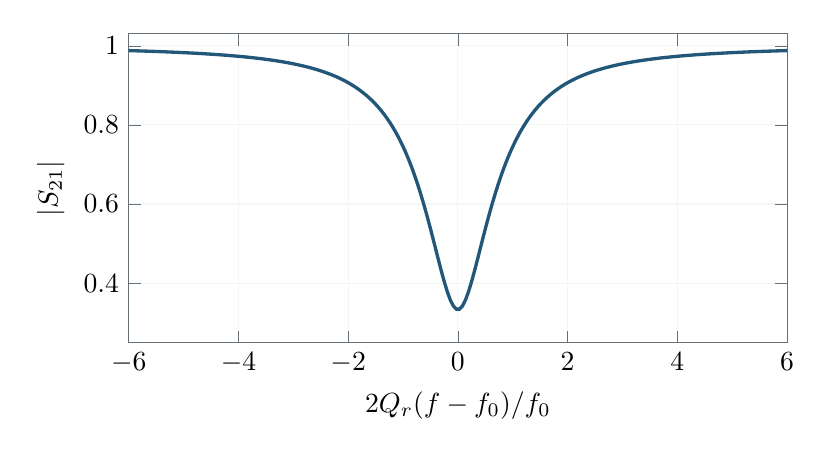
\begin{tikzpicture}
\begin{axis}[
  width=0.82\textwidth,height=5.5cm,
  xlabel={$2Q_r(f-f_0)/f_0$},ylabel={$|S_{21}|$},
  xmin=-6,xmax=6,ymin=0.25,ymax=1.03,
  grid=major,grid style={draw=KidGray},
  axis line style={draw=KidDark!70},tick style={draw=KidDark!70}
]
\addplot[KidBlue,very thick,domain=-6:6,samples=220]
  {sqrt(((1-0.6666667)^2+x^2)/(1+x^2))};
\end{axis}
\end{tikzpicture}
\end{center}

这里取 $Q_i=10^5,Q_c=5\times10^4$，因此 $d=Q_r/Q_c\approx2/3$。曲线的“深度”和“宽度”不是同一个信息：宽度主要给 $Q_r$，深度/圆直径再帮助分解 $Q_c$ 与 $Q_i$。

\section{为什么复数 $S_{21}$ 会形成一个圆？}

把上式分解成实部与虚部：
\[
\operatorname{Re}S_{21}=1-\frac{d}{1+y^2},
\qquad
\operatorname{Im}S_{21}=\frac{dy}{1+y^2}.
\]
消去 $y$ 可得
\[
\boxed{
\left(\operatorname{Re}S_{21}-\left(1-\frac d2\right)\right)^2
+
\left(\operatorname{Im}S_{21}\right)^2
=
\left(\frac d2\right)^2.
}
\]
因此理想 resonance 在 IQ 平面上严格是一条圆：
\begin{itemize}
  \item 圆心：$\left(1-d/2,0\right)$；
  \item 半径：$d/2$；
  \item far off resonance：$S_{21}\rightarrow1$；
  \item resonance point：$S_{21}(f_0)=1-d$。
\end{itemize}

\begin{center}
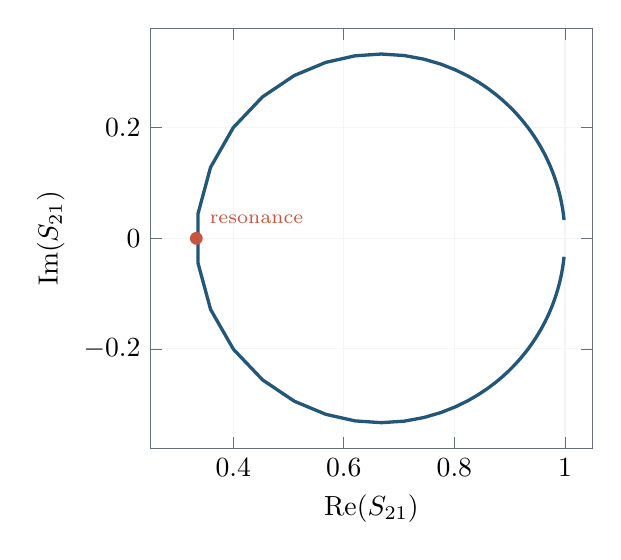
\begin{tikzpicture}
\begin{axis}[
  width=7.2cm,height=7.2cm,
  xlabel={Re$(S_{21})$},ylabel={Im$(S_{21})$},
  axis equal image,
  xmin=0.25,xmax=1.05,ymin=-0.38,ymax=0.38,
  grid=major,grid style={draw=KidGray},
  axis line style={draw=KidDark!70},tick style={draw=KidDark!70}
]
\addplot[KidBlue,very thick,domain=-20:20,samples=300,variable=\t]
  ({1-0.6666667/(1+\t^2)},{0.6666667*\t/(1+\t^2)});
\addplot[only marks,mark=*,mark size=2.1pt,KidRed] coordinates {(0.3333333,0)};
\node[font=\scriptsize,anchor=south west,text=KidRed] at (axis cs:0.34,0.01) {resonance};
\end{axis}
\end{tikzpicture}
\end{center}

这张圆不是画图技巧，而是一个非常有价值的拟合约束。真实 VNA 数据即使被放大、旋转、延迟，只要系统近似线性，resonance 轨迹仍然保留“圆结构”，这也是 circle fit 方法能够工作的原因。

\section{耦合强弱：不要只凭 notch 深浅判断“器件好不好”}

由
\[
\frac1{Q_r}=\frac1{Q_i}+\frac1{Q_c}
\]
可看出两种极限：

\subsection{$Q_c\gg Q_i$：feedline 耦合很弱}
此时
\[
Q_r\approx Q_i,
\qquad
\frac{Q_r}{Q_c}\ll1,
\]
因此 notch 很浅。器件可能内部损耗很低，也可能只是“几乎没耦合进去”。

\subsection{$Q_c\ll Q_i$：耦合损耗率占主导}
此时
\[
Q_r\approx Q_c,
\qquad
\frac{Q_r}{Q_c}\approx1,
\]
理想 lossless 极限下 resonance 可以接近零传输，notch 很深。

\begin{intuitionbox}
对于 hanger transmission geometry，与其在初学阶段机械套用“critical / under / over coupled”三个词，不如先问两个更不会错的问题：\textbf{内部损耗率大，还是 feedline 耦合率大？}以及\textbf{$Q_r$ 是被 $Q_i$ 限制，还是被 $Q_c$ 限制？}
\end{intuitionbox}

\section{KID 真正的读出：固定 probe tone，而不是不停扫 VNA}

扫频的主要作用是先找到 $f_0,Q_r,Q_c,Q_i$。真正观测时，我们通常在 resonance 附近固定一个或多个 readout tone，然后连续采集
\[
S_{21}(t)=I(t)+jQ(t).
\]

在一个工作点附近，可以线性化：
\[
\boxed{
\delta S_{21}
\approx
\frac{\partial S_{21}}{\partial f_0}\delta f_0
+
\frac{\partial S_{21}}{\partial(Q_i^{-1})}\delta(Q_i^{-1}).
}
\]
第一项主要来自 reactive / frequency response，第二项主要来自 dissipative response。

在 IQ 圆上可以形成一个很实用的几何直觉：
\begin{itemize}
  \item 改变 $f_0$，相当于让固定 probe tone 在 resonance 圆轨迹上“前后滑动”；
  \item 改变内部损耗，会同时改变圆的尺寸/位置和 probe point 到圆心的关系；
  \item 因而可以在局部定义近似正交的 frequency quadrature 与 dissipation quadrature。
\end{itemize}

\begin{center}
\begin{tikzpicture}[scale=1.05]
\draw[draw=KidDark!35] (0,0) circle (2.0cm);
\coordinate (C) at (0,0);
\coordinate (P) at (1.40,1.43);
\fill[KidBlue] (P) circle (2pt);
\draw[flowarrow] (P) -- ++(-0.72,0.70) node[above left,font=\scriptsize,text=KidBlue] {$\delta f_0$：沿切向为主};
\draw[goldarrow] (P) -- ++(0.72,0.72) node[above right,font=\scriptsize,text=KidGold!70!black] {$\delta Q_i^{-1}$：径向/形变为主};
\fill[KidDark] (C) circle (1.3pt) node[below,font=\scriptsize]{circle center};
\node[below right,font=\scriptsize,text=KidDark!70] at (P) {固定 probe 工作点};
\end{tikzpicture}
\end{center}

\begin{mistakebox}
“frequency direction 和 dissipation direction 永远严格正交”不是普遍定理。它们在经过正确归一化并在线性小信号附近可以构造为近似正交坐标；真实 cable delay、非对称耦合、噪声和非线性都会让几何关系偏离这张理想图。
\end{mistakebox}

\section{真实 VNA 数据为什么不是一个端正的圆？}

实验数据往往还叠加 readout chain：
\begin{itemize}
  \item cable delay 带来频率相关相位旋转；
  \item 放大器、衰减器、线缆带来 complex gain；
  \item 频率相关 baseline 让圆整体倾斜或拉伸；
  \item input/output impedance mismatch 可以产生 resonance asymmetry；
  \item 噪声让点云不再落在一条完美圆上。
\end{itemize}

一个常用的工程模型可以写成
\[
\boxed{
S_{21}^{\rm meas}(f)
=
G(f)e^{-j2\pi f\tau}
\left[
1-
\frac{(Q_r/Q_c)e^{j\phi}}
{1+2jQ_r(f-f_0)/f_0}
\right],
}
\]
其中
\begin{itemize}
  \item $G(f)$ 表示缓慢变化的 complex gain / baseline；
  \item $\tau$ 是 electrical delay；
  \item $\phi$ 是把 mismatch / asymmetry 吸收到一个有效复耦合角中的教学参数。
\end{itemize}

不同文献对 complex coupling quality factor 与 $\phi$ 的定义略有不同，所以真正复现 fitting code 时必须跟随所用模型的约定，不能只复制一个公式外形。

\section{一个可靠的 resonance fitting 流程}

面对一段真实 $S_{21}(f)$，建议按以下层级思考：

\begin{center}
\begin{tikzpicture}[node distance=7mm and 5mm]
\node[flowbox,fill=KidGray,minimum width=25mm] (raw) {raw complex\\$S_{21}(f)$};
\node[flowbox,right=of raw,minimum width=27mm] (delay) {估计/去除\\cable delay};
\node[flowbox,right=of delay,minimum width=28mm] (base) {complex gain\\baseline normalization};
\node[flowbox,right=of base,minimum width=27mm] (circle) {circle / line-shape\\fit};
\node[flowbox,right=of circle,minimum width=28mm] (par) {$f_0,Q_r,Q_c,Q_i$\\+ uncertainty};
\draw[flowarrow] (raw.east)--(delay.west);
\draw[flowarrow] (delay.east)--(base.west);
\draw[flowarrow] (base.east)--(circle.west);
\draw[flowarrow] (circle.east)--(par.west);
\end{tikzpicture}
\end{center}

最低限度的质量检查包括：
\begin{enumerate}
  \item 拟合残差是否随机，而不是还留着系统性弧形；
  \item 拟合窗口变宽/变窄时参数是否稳定；
  \item $Q_i,Q_c,Q_r$ 是否满足定义关系；
  \item 去 delay 前后 IQ 轨迹是否合理；
  \item 是否存在 nearby resonance、非线性、功率依赖或频率跳变。
\end{enumerate}

\section{为什么 resonance fitting 对 KID 比“普通滤波器”更重要？}

KID 的科学信号最终不是“有没有 notch”，而是小变化：
\[
\delta f_0(t),
\qquad
\delta Q_i^{-1}(t).
\]
如果 baseline、delay 或 coupling 模型错了，这些系统误差会直接投影成假的 optical response。

对于阵列还会进一步影响：
\begin{itemize}
  \item tone placement：probe tone 是否真的落在合适工作点；
  \item tone spacing：邻近 resonance 是否可能 collision；
  \item readout dynamic range：大量 tone 的 crest factor 与放大器线性区；
  \item tracking：光学负载变化后是否需要自动跟踪 $f_0$。
\end{itemize}

这就是为什么 $Q$、IQ circle 和 fitting 不是“读出工程的附属知识”，而是 detector calibration 本身。

\section{映射到你现在的 LEKID 仿真}

\begin{projectbox}
你目前 Sonnet 里更常看到的是 GHz resonance。下一步可以把仿真结果按三个层级拆开：
\begin{enumerate}
  \item \textbf{geometry level：}meander + IDC + coupling 共同决定 $L,C$ 与耦合强度；
  \item \textbf{resonator level：}从复数 $S_{21}$ 拟合 $f_0,Q_r,Q_c,Q_i$；
  \item \textbf{material / detector level：}只有当超导薄膜模型包含真实 $Z_s$ / $L_k$ / loss 时，$Q_i$ 与 $f_0$ 才能继续往材料参数和光学响应解释。
\end{enumerate}
因此以后不建议只报“谐振在 \SI{2.5}{GHz}、notch 很深”，而应至少输出 $f_0,Q_r,Q_c$，并说明 $Q_i$ 是否物理可信、材料模型是否允许解释它。
\end{projectbox}

\section{v0.5 配套 Python：从理想 resonance 到带失真的 synthetic VNA}

本版本仓库新增两个可直接运行的示例：
\begin{itemize}
  \item \texttt{examples/v0.5/resonator\_basics.py}：生成理想 notch、IQ circle、光照导致的 $f_0$ 位移与固定 tone IQ 位移；
  \item \texttt{examples/v0.5/resonator\_fit\_demo.py}：给理想 resonance 加入 complex gain、cable delay、asymmetry 和复高斯噪声，再用非线性 least-squares 拟合回 $f_0,Q_r,Q_c,\phi,\tau$ 等参数。
\end{itemize}

建议先不看 fitting 脚本实现，自己完成第一个脚本中的四个 TODO，再运行参考版本对照。

\section{本章 2--3 小时学习任务}

\begin{enumerate}
  \item 从 $Q=\omega_0U/P_{loss}$ 独立推导 $1/Q_r=1/Q_i+1/Q_c$；
  \item 用 $f_0=\SI{2.5}{GHz},Q_i=10^5,Q_c=5\times10^4$ 算出 $Q_r,\Delta f,\tau_E,\tau_A$；
  \item 从 ideal $S_{21}$ 推导 IQ 圆方程，亲手证明圆心为 $1-d/2$、半径为 $d/2$；
  \item 运行 \texttt{resonator\_basics.py}，改变 $Q_i/Q_c$，观察 notch depth、linewidth 和圆直径分别怎么变化；
  \item 将 $f_0$ 人为移动 $-10$、$-30$、$-100\,\mathrm{kHz}$，比较固定 probe tone 的 $\Delta I,\Delta Q$；
  \item 运行 synthetic fitting 示例，分别关掉 cable delay、asymmetry、noise，观察每一种非理想项对 recovered $Q_i$ 的影响；
  \item 最后闭卷回答：\textbf{为什么只看 $|S_{21}|$ 不如同时拟合复数 $S_{21}$？}
\end{enumerate}

\section{闭卷理解检查}

\begin{checkpointbox}
\begin{enumerate}
  \item $Q_i,Q_c,Q_r$ 分别对应什么物理通道？
  \item 为什么独立损耗通道是 $1/Q$ 相加，而不是 $Q$ 相加？
  \item $Q_r$ 增大一倍时 linewidth 如何变化？
  \item energy lifetime 与 amplitude lifetime 为什么相差 2？
  \item ideal hanger $S_{21}$ 为什么在复平面是一条圆？
  \item notch 很浅时，为什么不能立刻判断器件内部损耗很大？
  \item 固定 probe tone 为什么能把 $\delta f_0$ 变成 $\delta I,\delta Q$？
  \item cable delay 在 IQ 平面最主要造成什么变化？
  \item 为什么 resonance asymmetry 会让简单的“旋转圆”方法偏置 $Q_i$？
  \item 对你当前 Sonnet 结果，哪些 $Q$ 可以直接从 $S_{21}$ 得到，哪些解释依赖真实超导材料模型？
\end{enumerate}
\end{checkpointbox}

\begin{formula}[title=\bfseries 本章的一句话]
\centering
\[
\boxed{
(Q_i,Q_c)
\rightarrow
Q_r
\rightarrow
(\Delta f,\tau)
\rightarrow
S_{21}(f)
\rightarrow
\text{IQ circle}
\rightarrow
\text{fixed-tone }I/Q
}
\]
\end{formula}


\chapter{光学响应、噪声与 NEP：把“看到光”变成一个可比较的灵敏度指标}

\begin{goalbox}
学完本章后，你应该能够把一颗 KID 的光学响应写成一条可计算的链：
\[
P_{\rm abs}\rightarrow \Gamma_{\rm qp}\rightarrow N_{\rm qp}\rightarrow
\delta f_0,\delta Q_i^{-1}\rightarrow \delta I,\delta Q,
\]
并能够回答：
\begin{enumerate}
  \item responsivity 到底是“对什么量求导”；
  \item 为什么 quasiparticle lifetime 同时决定信号增益和响应速度；
  \item PSD、ASD 与 NEP 的单位分别是什么；
  \item photon、generation--recombination、TLS、amplifier noise 在频谱上通常长什么样；
  \item 怎样判断一颗 KID 是否接近 photon-noise limited。
\end{enumerate}
\end{goalbox}

\section{先把这一章放回整条 KID 链}

前五个版本主要解决了“材料变化怎样变成 GHz 复数 $S_{21}$”。本章第一次把输入端的光功率和输出端的噪声统一起来：

\begin{center}
\begin{tikzpicture}[node distance=9mm and 7mm]
\node[flowbox,fill=KidGold!22,minimum width=27mm] (p) {$P_{\rm abs}$\\吸收光功率};
\node[flowbox,right=of p,minimum width=29mm] (g) {$\Gamma_{\rm qp}$\\准粒子产生率};
\node[flowbox,right=of g,minimum width=27mm] (n) {$N_{\rm qp}$\\稳态与涨落};
\node[flowbox,right=of n,minimum width=31mm] (r) {$f_0,Q_i$\\谐振器响应};
\node[flowbox,right=of r,minimum width=28mm] (iq) {$I,Q$\\数字读出};
\draw[goldarrow] (p.east)--(g.west);
\draw[flowarrow] (g.east)--(n.west);
\draw[flowarrow] (n.east)--(r.west);
\draw[flowarrow] (r.east)--(iq.west);
\node[flowbox,fill=KidRed!5,below=14mm of n,text width=38mm] (noise) {随机涨落\\photon / GR / TLS / amplifier};
\draw[influence] (noise.north) -- (n.south);
\draw[influence] (noise.north east) to[bend left=18] (iq.south west);
\end{tikzpicture}
\end{center}

\begin{intuitionbox}
responsivity 回答的是“输入改变一点，输出平均值改变多少”；noise 回答的是“即使输入不变，输出自己会抖多少”。NEP 做的事情，就是把输出端的抖动除以 responsivity，重新折算成输入端等效的功率抖动。
\end{intuitionbox}

\section{从吸收光功率到 quasiparticle generation rate}

设真正沉积在超导吸收体中的功率为 $P_{\rm abs}$。注意它已经包含了光学链上的耦合、反射、偏振匹配等结果，不应与望远镜口径处的 incident power 混为一谈。

光子能量最终只有一部分进入可观测的 quasiparticle population。用 pair-breaking efficiency $\eta_{\rm pb}$ 表示这一比例。若每个 quasiparticle 的典型激发能量尺度取 $\Delta$，最常用的工程近似是
\[
\boxed{\Gamma_{\rm qp}\simeq \frac{\eta_{\rm pb}P_{\rm abs}}{\Delta}}
\]
其中 $\Gamma_{\rm qp}$ 的单位是 \si{s^{-1}}。

这个式子不要误读为“一个光子只产生一个 quasiparticle”。一个高于 $2\Delta$ 的光子会触发 pair breaking 和后续 phonon cascade；$\eta_{\rm pb}$ 把复杂能量级联压缩成一个有效参数。

\begin{mistakebox}
$P_{\rm abs}$、incident optical power 和 readout microwave power 是三种不同的功率。前两者属于被探测的光学链，最后一个是 GHz probe tone。把它们混写成一个 $P$ 是 KID 推导里很常见的错误。
\end{mistakebox}

\section{稳态 quasiparticle 数：为什么 lifetime 会提高响应}

在小扰动附近，可以把复杂的 recombination 动力学线性化为
\[
\frac{dN_{\rm qp}}{dt}=\Gamma_{\rm qp}-\frac{N_{\rm qp}-N_{\rm qp,0}}{\tau_{\rm qp}}.
\]
若只关注额外光生 population，并假设 $\tau_{\rm qp}$ 在工作点附近近似常数，则稳态有
\[
\boxed{
\delta N_{\rm qp}
\simeq
\frac{\eta_{\rm pb}\tau_{\rm qp}}{\Delta}
\,\delta P_{\rm abs}
}
\]
于是
\[
\boxed{
\frac{\partial N_{\rm qp}}{\partial P_{\rm abs}}
\simeq
\frac{\eta_{\rm pb}\tau_{\rm qp}}{\Delta}
}
\]

这给出一个非常重要的器件直觉：\textbf{更长的 $\tau_{\rm qp}$ 会让同样的光功率在器件里积累更多 quasiparticle，因此静态 responsivity 往往更高。}

但它不是免费的，因为更长的 lifetime 同时意味着更慢的响应。

\section{从 $N_{\rm qp}$ 到 frequency / dissipation responsivity}

定义 fractional frequency shift
\[
x\equiv \frac{\delta f_0}{f_0}.
\]
在某个固定工作点附近，先不强迫自己每次都重新计算完整 Mattis--Bardeen 积分，而是定义材料-几何转换系数
\[
\mathcal K_x\equiv \frac{\partial x}{\partial N_{\rm qp}},
\qquad
\mathcal K_d\equiv
\frac{\partial Q_i^{-1}}{\partial N_{\rm qp}}.
\]
对于通常的 KID，$\mathcal K_x<0$，因为 quasiparticle 增多导致 $\sigma_2$ 下降、$L_k$ 增大、$f_0$ 下降；而 $\mathcal K_d>0$，因为耗散增加。

于是光功率 responsivity 为
\[
\boxed{
\mathcal R_x
\equiv
\frac{\partial x}{\partial P_{\rm abs}}
=\mathcal K_x
\frac{\eta_{\rm pb}\tau_{\rm qp}}{\Delta}
}
\]
以及
\[
\boxed{
\mathcal R_d
\equiv
\frac{\partial Q_i^{-1}}{\partial P_{\rm abs}}
=\mathcal K_d
\frac{\eta_{\rm pb}\tau_{\rm qp}}{\Delta}
}.
\]

如果需要更显式地接回 Mattis--Bardeen，常见小信号形式可写成
\[
\frac{\delta f_0}{f_0}
\propto
-\frac{\alpha S_2}{N_0\Delta V}\,\delta N_{\rm qp},
\]
\[
\delta Q_i^{-1}
\propto
\frac{\alpha S_1}{N_0\Delta V}\,\delta N_{\rm qp},
\]
其中 $S_1,S_2$ 是由温度与读出频率决定的 Mattis--Bardeen response factors。不同文献对 $N_0$、spin degeneracy 和几何因子约定不同，因此第一次使用具体 prefactor 时一定核对定义。

\section{再往前一步：从 responsivity 到真正的 $I/Q$ responsivity}

上一章已经有
\[
\delta S_{21}
\simeq
\frac{\partial S_{21}}{\partial f_0}\delta f_0
+
\frac{\partial S_{21}}{\partial Q_i^{-1}}\delta Q_i^{-1}.
\]
因此
\[
\boxed{
\frac{\partial S_{21}}{\partial P_{\rm abs}}
=
\frac{\partial S_{21}}{\partial f_0}
\frac{\partial f_0}{\partial P_{\rm abs}}
+
\frac{\partial S_{21}}{\partial Q_i^{-1}}
\frac{\partial Q_i^{-1}}{\partial P_{\rm abs}}
}
\]
就是 fixed-tone readout 最直接的复数 responsivity。

写成
\[
S_{21}=I+jQ,
\]
就得到两个实数：
\[
\mathcal R_I=\frac{\partial I}{\partial P_{\rm abs}},
\qquad
\mathcal R_Q=\frac{\partial Q}{\partial P_{\rm abs}}.
\]
工程上更常做的是先把 $(I,Q)$ 旋转到 frequency / dissipation 两个近似正交的坐标，再在这两个坐标里分别做 responsivity 和 noise analysis。

\section{时间响应：$\tau_{\rm qp}$ 与 resonator ring-down 谁更慢？}

若 optical power 有一个小的正弦调制 $\delta P e^{j2\pi ft}$，quasiparticle population 的一阶响应是
\[
H_{\rm qp}(f)=\frac{1}{1+j2\pi f\tau_{\rm qp}}.
\]
对应的 $-3\,\mathrm{dB}$ 截止频率：
\[
\boxed{f_{\rm qp}=\frac{1}{2\pi\tau_{\rm qp}}}.
\]

但读出端的 resonator 自己也有有限 ring-down。用上一章的 amplitude lifetime
\[
\tau_A=\frac{2Q_r}{\omega_0}
=\frac{Q_r}{\pi f_0},
\]
可把其基带响应也近似成一个低通环节。

因此一个最小动态模型是
\[
H_{\rm det}(f)
\simeq
\frac{1}{1+j2\pi f\tau_{\rm qp}}
\frac{1}{1+j2\pi f\tau_A}.
\]

\begin{projectbox}
假设你的读出 resonance 在 \SI{2.5}{GHz}，$Q_r=3.3\times10^4$，则 $\tau_A\approx\SI{4.2}{\micro s}$；若低温 Al 的有效 quasiparticle lifetime 是 \SI{300}{\micro s}，那么 detector bandwidth 主要由 quasiparticle 动力学而不是 resonator 限制。反过来，如果未来做极快 pulse detector 或故意把 $Q_r$ 做得非常高，ring-down 就可能进入瓶颈。
\end{projectbox}

\section{Noise PSD 与 ASD：先把单位彻底理顺}

若某个读出量 $y(t)$ 的单边功率谱密度记作 $S_y(f)$，单位是
\[
[y]^2/\mathrm{Hz}.
\]
其 amplitude spectral density 是
\[
\sqrt{S_y(f)},
\]
单位是
\[
[y]/\sqrt{\mathrm{Hz}}.
\]

例如 fractional frequency noise
\[
x(t)=\frac{\delta f_0(t)}{f_0}
\]
是无量纲量，因此
\[
S_x(f):\quad \mathrm{Hz}^{-1},
\qquad
\sqrt{S_x(f)}:\quad \mathrm{Hz}^{-1/2}.
\]

若直接用 frequency fluctuation $\delta f_0(t)$，则
\[
\sqrt{S_f}:\quad \mathrm{Hz}/\sqrt{\mathrm{Hz}}.
\]

\section{NEP：把输出噪声折回输入端}

如果选择 $x=\delta f_0/f_0$ 作为 detector observable，则
\[
\mathcal R_x=\frac{dx}{dP_{\rm abs}}
\]
单位为 \si{W^{-1}}。于是 input-referred NEP 定义为
\[
\boxed{
\mathrm{NEP}(f)
=
\frac{\sqrt{S_x(f)}}{|\mathcal R_x(f)|}
}
\]
单位自然是
\[
\boxed{\mathrm{W}/\sqrt{\mathrm{Hz}}}.
\]

同理，如果你使用 phase、$I$、$Q$ 或 dissipation channel，只要 noise 和 responsivity 使用同一个 observable，最后都可以换算成 NEP。

\begin{intuitionbox}
NEP 不是“输出噪声有多小”，而是“多小的输入功率涨落能够产生和现有输出噪声一样大的信号”。因此没有 responsivity，单独报一个 IQ noise 数字并不能说明 detector 灵敏度。
\end{intuitionbox}

\section{Photon noise：输入光本身就是随机的}

对于中心频率 $\nu$、吸收功率 $P_{\rm abs}$、等效光学带宽 $\Delta\nu$ 的单模近似，常见表达式是
\[
\boxed{
\mathrm{NEP}_{\rm ph}^2
\simeq
2h\nu P_{\rm abs}
+
\frac{2P_{\rm abs}^2}{\Delta\nu}
}
\]
第一项是 photon shot noise，第二项来自 thermal bunching / wave noise。

在低 occupancy 条件下，第一项常占主导：
\[
\mathrm{NEP}_{\rm shot}
\simeq
\sqrt{2h\nu P_{\rm abs}}.
\]

真正的多模、多偏振、宽带系统需要对 bandpass 和 occupation number 积分；上式的作用是建立量级和物理来源，而不是替代完整 optical model。

\section{Generation--recombination noise：quasiparticle 数自己也会涨落}

quasiparticle 的产生和复合是随机过程，因此即使平均 $N_{\rm qp}$ 不变，也会有 number fluctuation。在线性化模型和一种常用单边 PSD 约定下，低频 quasiparticle-number noise 可写为
\[
S_N(f)
\simeq
\frac{4N_{\rm qp}\tau_{\rm qp}}
{1+(2\pi f\tau_{\rm qp})^2}.
\]

利用
\[
\frac{dN_{\rm qp}}{dP_{\rm abs}}
\simeq
\frac{\eta_{\rm pb}\tau_{\rm qp}}{\Delta},
\]
可得到低频 input-referred GR noise 的常见形式
\[
\boxed{
\mathrm{NEP}_{\rm GR}
\simeq
\frac{2\Delta}{\eta_{\rm pb}}
\sqrt{\frac{N_{\rm qp}}{\tau_{\rm qp}}}
}.
\]
如果 quasiparticle population 主要由该 optical load 产生，并使用前述线性稳态关系，则进一步有
\[
\mathrm{NEP}_{\rm GR}^2
\simeq
\frac{4\Delta P_{\rm abs}}{\eta_{\rm pb}}.
\]
不同文献对 one-sided / two-sided PSD、$N_0$ 和 generation event 的定义会带来 factor-of-two 差别，所以比较数值时必须先对齐 convention。

\section{TLS noise：为什么低频 frequency channel 常常变“粉红”}

Two-Level Systems 通常与非晶介质、界面、电场集中的 capacitor 区域有关。它对 KID 最典型的影响不是简单增加一个白噪声底，而是造成低频 excess frequency noise，经验上常近似写作
\[
S_x^{\rm TLS}(f)\propto f^{-\beta},
\qquad \beta\sim 0.5\text{--}1,
\]
具体指数依器件、温度与 readout power 而变。

TLS 噪声通常具有几个工程特征：
\begin{itemize}
  \item 在低 Fourier frequency 更强；
  \item 对 capacitor 电场分布和介质参与比敏感；
  \item 增加 readout power 往往能在一定范围内使 TLS 饱和、降低其相对噪声；
  \item 但 readout power 过高又会进入 kinetic-inductance nonlinearity、heating 或 bifurcation。
\end{itemize}

这也是为什么 IDC 几何不是只负责“把谐振频率调到某个 GHz”，它还可能直接影响最终 noise floor。

\section{Amplifier / readout noise：它发生在 detector 之后}

低温 HEMT、室温放大器、ADC 量化与数字链都会给 $I/Q$ 添加噪声。理想放大器噪声在窄带基带里通常近似为白噪声。

它与 photon / GR noise 的关键区别是：\textbf{它并没有真的改变 $N_{\rm qp}$，而是污染了我们对 $S_{21}$ 的测量。}

因此 input-referred amplifier NEP 应写成
\[
\mathrm{NEP}_{\rm amp}(f)
=
\frac{\sqrt{S_{y,\rm amp}(f)}}
{|dy/dP_{\rm abs}|},
\]
其中 $y$ 可以选 frequency quadrature、phase 或某个最优线性组合。

提高 readout power 可以改善 amplifier-limited SNR，但最终会受到 resonator nonlinearity 和 detector back-action 的限制，所以“readout tone 越强越好”是不成立的。

\section{一个 150 GHz Al LEKID 的量级例子}

取一个用于建立量级感的工作点：
\[
\nu=\SI{150}{GHz},\qquad
T_c=\SI{1.2}{K},\qquad
P_{\rm abs}=\SI{1}{pW},
\]
\[
\eta_{\rm pb}=0.57,\qquad
\tau_{\rm qp}=\SI{300}{\micro s}.
\]
弱耦合 BCS 给出
\[
\Delta\simeq1.764k_BT_c\simeq\SI{0.182}{meV}.
\]
于是线性稳态估计
\[
N_{\rm qp}
\simeq
\frac{\eta_{\rm pb}P_{\rm abs}\tau_{\rm qp}}{\Delta}
\approx 5.9\times10^6.
\]

photon shot-noise 量级：
\[
\mathrm{NEP}_{\rm shot}
\approx
\sqrt{2h\nu P_{\rm abs}}
\approx
1.4\times10^{-17}\,\mathrm{W}/\sqrt{\mathrm{Hz}}.
\]
在相同近似与 PSD convention 下，GR noise 也得到约
\[
\mathrm{NEP}_{\rm GR}
\approx
1.4\times10^{-17}\,\mathrm{W}/\sqrt{\mathrm{Hz}}.
\]

这个“恰好同量级”不是所有 KID 的普遍定律，但它说明：在设计得不错的 pair-breaking detector 中，GR noise 本来就可能靠近 photon noise，而不是比它小很多个数量级。

\section{怎样做真正的 noise budget？}

如果各噪声源近似独立，则 input-referred noise 可按功率相加：
\[
\boxed{
\mathrm{NEP}_{\rm tot}^2(f)
=
\mathrm{NEP}_{\rm ph}^2
+
\mathrm{NEP}_{\rm GR}^2
+
\mathrm{NEP}_{\rm TLS}^2(f)
+
\mathrm{NEP}_{\rm amp}^2(f)
+\cdots
}
\]

工程上不应该只给一个“最小 NEP”，而应画出 NEP versus Fourier frequency。因为 detector 可能在 \SI{100}{Hz} 附近 photon-noise limited，却在 \SI{0.1}{Hz} 被 TLS / $1/f$ drift 完全支配。

\begin{center}
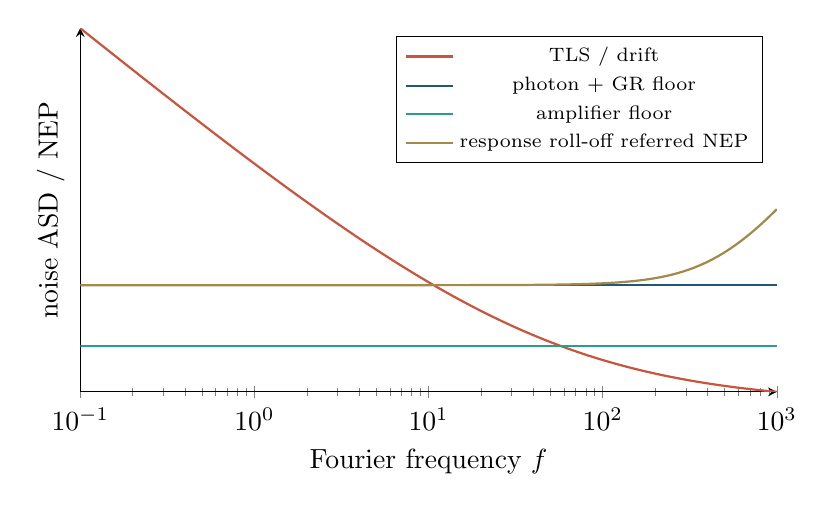
\begin{tikzpicture}
\begin{axis}[
width=0.86\textwidth,height=6.2cm,
xmode=log,ymode=log,
xlabel={Fourier frequency $f$},ylabel={noise ASD / NEP},
xtick={0.1,1,10,100,1000},
ytick=\empty,
legend style={font=\scriptsize,at={(0.98,0.98)},anchor=north east},
axis lines=left]
\addplot[KidRed,thick,domain=0.1:1000,samples=120] {1.4/x^0.65+0.12};
\addlegendentry{TLS / drift}
\addplot[KidBlue,thick,domain=0.1:1000,samples=80] {0.42};
\addlegendentry{photon + GR floor}
\addplot[KidTeal,thick,domain=0.1:1000,samples=80] {0.22};
\addlegendentry{amplifier floor}
\addplot[KidGold!70!black,thick,domain=0.1:1000,samples=120] {0.42*sqrt(1+(x/500)^2)};
\addlegendentry{response roll-off referred NEP}
\end{axis}
\end{tikzpicture}
\end{center}

这张图是概念示意，不对应某个具体器件；它要表达的是：\textbf{“噪声大小”必须和 Fourier frequency 绑定。}

\section{什么叫 photon-noise limited？}

一个实用判据不是“总 NEP 等于理论 photon NEP 到最后一位”，而是在目标科学频带内满足
\[
\mathrm{NEP}_{\rm other}^2
\ll
\mathrm{NEP}_{\rm ph}^2,
\]
使得
\[
\mathrm{NEP}_{\rm tot}
\approx
\mathrm{NEP}_{\rm ph}
\]
并且随着 optical loading 变化呈现合理的 photon-noise scaling。

真正有说服力的验证通常包括：
\begin{enumerate}
  \item blackbody / optical load 改变时测 $f_0$ 与 $Q_i$，得到 responsivity；
  \item 对同一工作点记录长时间 $I/Q$ timestream；
  \item 转成 frequency / dissipation noise PSD；
  \item 用 measured responsivity 折算 NEP；
  \item 与 photon + GR + readout noise model 比较；
  \item 改变 optical loading、bath temperature 和 readout power，检查 scaling 是否一致。
\end{enumerate}

\section{映射到你的双偏振 150 GHz LEKID 项目}

\begin{projectbox}
对于你当前器件，v0.6 以后可以把“好不好”拆成四层，不再只看 absorption 或 notch：
\begin{enumerate}
  \item \textbf{Optical layer：}$A_X(\nu,\theta),A_Y(\nu,\theta)$，得到每个偏振真正的 $P_{\rm abs}$；
  \item \textbf{Material layer：}$P_{\rm abs}\rightarrow N_{\rm qp}\rightarrow\delta\sigma_1,\delta\sigma_2$；
  \item \textbf{Resonator layer：}$\delta\sigma\rightarrow\delta f_0,\delta Q_i^{-1}\rightarrow\delta I/Q$；
  \item \textbf{Sensitivity layer：}responsivity + noise PSD $\rightarrow$ NEP。
\end{enumerate}
这意味着你未来比较 B0 / B1 backshort 时，最终可以问的不只是“谁吸收率高”，还可以问“谁在给定 sky loading 下得到更优、且偏振更对称的 end-to-end responsivity / NEP”。这会比单纯的电磁吸收比较更像一个完整 detector 研究问题。
\end{projectbox}

\section{v0.6 配套 Python}

本版本增加两个示例：
\begin{itemize}
  \item \texttt{docs/v0.6/examples/optical\_responsivity\_demo.py}：从 $P_{\rm abs}$ 计算 $N_{\rm qp}$，再用一个可替换的 $dx/dN_{\rm qp}$ calibration coefficient 生成 fractional frequency response，并画出 quasiparticle lifetime 对响应速度的影响；
  \item \texttt{docs/v0.6/examples/noise\_budget\_demo.py}：计算 150 GHz 下的 photon shot / bunching noise、GR noise，并演示如何把一个 measured fractional-frequency noise ASD 用 responsivity 折算成 NEP。
\end{itemize}

\section{本章 3--4 小时学习任务}

\begin{enumerate}
  \item 从 $\Gamma_{\rm qp}=\eta_{\rm pb}P_{\rm abs}/\Delta$ 和一阶 lifetime 模型推导 $dN_{\rm qp}/dP_{\rm abs}$；
  \item 用本章 Al 数值例子独立算一遍 $\Delta,N_{\rm qp},\mathrm{NEP}_{\rm shot},\mathrm{NEP}_{\rm GR}$；
  \item 证明 NEP 的单位一定是 \si{W/\sqrt{Hz}}；
  \item 画出 $|H_{\rm qp}(f)|$，把 $\tau_{\rm qp}$ 从 \SI{30}{\micro s} 改到 \SI{3}{ms}，观察 bandwidth；
  \item 假设一个 measured $\sqrt{S_x}=10^{-9}/\sqrt{\mathrm{Hz}}$ 和 $|dx/dP|=10^6\,\mathrm{W^{-1}}$，计算 detector NEP；
  \item 运行 noise budget 脚本，改变 $P_{\rm abs}$ 与 $\Delta\nu$，观察 shot / bunching / GR 三项怎样缩放；
  \item 最后闭卷回答：\textbf{为什么“响应很大”不等于“NEP 很好”？}
\end{enumerate}

\section{闭卷理解检查}

\begin{checkpointbox}
\begin{enumerate}
  \item $\eta_{\rm pb}$ 在物理上压缩了哪些复杂过程？
  \item 为什么 $\tau_{\rm qp}$ 增大会提高静态 responsivity，却降低动态带宽？
  \item frequency responsivity 与 $I/Q$ responsivity 有什么区别？
  \item PSD 和 ASD 的单位为什么相差一个平方根？
  \item NEP 为什么必须通过同一 observable 的 responsivity 来 input-refer？
  \item photon shot noise 与 bunching noise 分别怎样随 $P_{\rm abs}$ 缩放？
  \item GR noise 是发生在 readout amplifier 之前还是之后？
  \item TLS 为什么经常首先污染低 Fourier frequency 的 frequency channel？
  \item 为什么提高 readout power 可以改善 amplifier-limited SNR，却不能无限提高？
  \item 你要证明一颗 KID photon-noise limited，至少需要做哪些 loading / PSD / responsivity 测量？
\end{enumerate}
\end{checkpointbox}

\begin{formula}[title=\bfseries 本章的一句话]
\centering
\[
\boxed{
P_{\rm abs}
\rightarrow N_{\rm qp}
\rightarrow (f_0,Q_i)
\rightarrow I/Q,
\qquad
\mathrm{NEP}=\frac{\text{output noise ASD}}{\text{responsivity}}
}
\]
\end{formula}


\chapter*{后续版本计划}
\addcontentsline{toc}{chapter}{后续版本计划}
\begin{itemize}
  \item v0.7：LEKID absorber / IDC / coupling / polarization / backshort 的电磁设计；
  \item v0.8：把上述理论逐项映射到当前双偏振 \SI{150}{GHz} LEKID 项目与 Sonnet/CST 验证矩阵，并加入 Python 数值练习。
\end{itemize}

\chapter*{建议参考资料}
\addcontentsline{toc}{chapter}{建议参考资料}
\begin{enumerate}
  \item P. K. Day et al., ``A broadband superconducting detector suitable for use in large arrays,'' \textit{Nature}, 425, 817--821 (2003).
  \item S. Doyle, \textit{Lumped Element Kinetic Inductance Detectors}, PhD thesis, Cardiff University (2008).
  \item J. Zmuidzinas, ``Superconducting Microresonators: Physics and Applications,'' \textit{Annual Review of Condensed Matter Physics}, 3, 169--214 (2012).
  \item J. Gao, \textit{The Physics of Superconducting Microwave Resonators}, PhD thesis, California Institute of Technology (2008).
  \item M. Tinkham, \textit{Introduction to Superconductivity}, 2nd ed., McGraw--Hill (1996).
  \item S. B. Kaplan et al., ``Quasiparticle and phonon lifetimes in superconductors,'' \textit{Physical Review B}, 14, 4854--4873 (1976).
  \item A. Rothwarf and B. N. Taylor, ``Measurement of Recombination Lifetimes in Superconductors,'' \textit{Physical Review Letters}, 19, 27--30 (1967).
  \item P. J. de Visser et al., ``Generation-Recombination Noise: The Fundamental Sensitivity Limit for Kinetic Inductance Detectors,'' \textit{Journal of Low Temperature Physics}, 167, 335--340 (2012).
  \item D. C. Mattis and J. Bardeen, ``Theory of the Anomalous Skin Effect in Normal and Superconducting Metals,'' \textit{Physical Review}, 111, 412--417 (1958).
  \item M. S. Khalil et al., ``An analysis method for asymmetric resonator transmission applied to superconducting devices,'' \textit{Journal of Applied Physics}, 111, 054510 (2012), doi:10.1063/1.3692073.
  \item S. Probst et al., ``Efficient and robust analysis of complex scattering data under noise in microwave resonators,'' \textit{Review of Scientific Instruments}, 86, 024706 (2015), doi:10.1063/1.4907935.
  \item P. J. de Visser et al., ``Evidence of a Nonequilibrium Distribution of Quasiparticles in the Microwave Response of a Superconducting Aluminum Resonator,'' \textit{Physical Review Letters}, 112, 047004 (2014).
  \item P. K. Day et al. and J. Zmuidzinas review sections on optical responsivity and noise are recommended as cross-checks for PSD/NEP conventions.
\end{enumerate}

\end{document}
